%\iffalse
% probsoln.dtx generated using makedtx version 0.94b (c) Nicola Talbot
% Command line args:
%   -macrocode ".+\.tex"
%   -comment ".+\.tex"
%   -src "(.+)\.(sty)\Z=>\1.\2"
%   -src "(sample.*)\.(tex)\Z=>\1.\2"
%   -src "(prob-.*)\.(tex)\Z=>\1.\2"
%   -doc "probsoln-manual.tex"
%   -author "Nicola Talbot"
%   probsoln
% Created on 2013/3/13 15:28
%\fi
%\iffalse
%<*package>
%% \CharacterTable
%%  {Upper-case    \A\B\C\D\E\F\G\H\I\J\K\L\M\N\O\P\Q\R\S\T\U\V\W\X\Y\Z
%%   Lower-case    \a\b\c\d\e\f\g\h\i\j\k\l\m\n\o\p\q\r\s\t\u\v\w\x\y\z
%%   Digits        \0\1\2\3\4\5\6\7\8\9
%%   Exclamation   \!     Double quote  \"     Hash (number) \#
%%   Dollar        \$     Percent       \%     Ampersand     \&
%%   Acute accent  \'     Left paren    \(     Right paren   \)
%%   Asterisk      \*     Plus          \+     Comma         \,
%%   Minus         \-     Point         \.     Solidus       \/
%%   Colon         \:     Semicolon     \;     Less than     \<
%%   Equals        \=     Greater than  \>     Question mark \?
%%   Commercial at \@     Left bracket  \[     Backslash     \\
%%   Right bracket \]     Circumflex    \^     Underscore    \_
%%   Grave accent  \`     Left brace    \{     Vertical bar  \|
%%   Right brace   \}     Tilde         \~}
%</package>
%\fi
% \iffalse
% Doc-Source file to use with LaTeX2e
% Copyright (C) 2013 Nicola Talbot, all rights reserved.
% \fi
% \iffalse
%<*driver>
\documentclass[a4paper]{nlctdoc}

\usepackage[utf8]{inputenc}
\usepackage[T1]{fontenc}
\usepackage{lmodern}
\usepackage{color}

\usepackage{probsoln}

\usepackage[colorlinks,
            bookmarks,
            hyperindex=false,
            pdfauthor={Nicola L.C. Talbot},
            pdftitle={probsoln: creating problem sheets optionally with solutions}]{hyperref}
\doxitem{Option}{option}{package options}

\RecordChanges
\PageIndex
\CheckSum{1822}

\newcommand*{\dq}[1]{``#1''}

\begin{document}
\DocInput{probsoln.dtx}
\end{document}
%</driver>
%\fi
%\MakeShortVerb{"}
%\DeleteShortVerb{\|}
%
% \title{probsoln v3.04: 
%creating problem sheets optionally with solutions}
% \author{Nicola L.C. Talbot\\[10pt]
%School of Computing Sciences\\
%University of East Anglia\\
%Norwich. Norfolk\\
%NR4 7TJ. United Kingdom.\\
%\url{http://theoval.cmp.uea.ac.uk/~nlct/}}
%
% \date{2012-08-23}
% \maketitle
%\tableofcontents
%
% \section{Introduction}
%The \styfmt{probsoln} package is designed for teachers or lecturers
%who want to create problem sheets for their students. This package
%was designed with mathematics problems in mind, but can be used for
%other subjects as well. The idea is to create a file containing a
%large number of problems with their solutions which can be read in
%by \LaTeX, and then select a number of problems to typeset. This
%means that once the database has been set up, each year you can
%easily create a new problem sheet that is sufficiently different
%from the previous year, thus preventing the temptation of current
%students seeking out the previous year's students, and checking out
%their answers. There is also an option that can be passed to the
%package to determine whether or not the solutions should be printed.
%In this way, one file can either produce the student's version or
%the teacher's version.
%
%\section{Package Options}\label{sec:pkgopt}
%The following options may be passed to this package:
%\begin{description}
%\item[\pkgopt{answers}]  Show the answers
%\item[\pkgopt{noanswers}] Don't show the answers (default)
%\item[\pkgopt{draft}] Display the label and dataset name when a problem is used
%\item[\pkgopt{final}] Don't display label and dataset name when a problem is used
%\item[\pkgopt{usedefaultargs}] Make \ics{thisproblem} use the
%default arguments supplied in the problem definition.
%\item[\pkgopt{nousedefaultargs}] Make \ics{thisproblem} prompt for
%problem arguments (default).
%\end{description}
%
%\section{Verbatim}\label{sec:verbatim}
%
%As from version 3.02, problems and solutions may contain verbatim
%text, but you must use the \iterm{fragile}\texttt{fragile} (or
%\texttt{fragile=true}) option for the associated environments.
%
%Alternatively, if most of your problems contain verbatim, you can
%globally set this option using:
%\begin{verbatim}
%\setkeys{probsoln}{fragile}
%\end{verbatim}
%You can switch off this option using \texttt{fragile=false}.
%
%The \texttt{fragile} option writes information to a temporary file.
%This defaults to "\jobname.vrb" but the name may be changed. The
%extension (".vrb") is given by:
%\begin{definition}[\DescribeMacro{\ProbSolnFragileExt}]
%\cs{ProbSolnFragileExt}
%\end{definition}
%The base name (\cs{jobname}) is given by:
%\begin{definition}[\DescribeMacro{\ProbSolnFragileFile}]
%\cs{ProbSolnFragileFile}
%\end{definition}
%
%\section{Showing and Hiding Solutions}\label{sec:showanswers}
%
%In addition to the \pkgopt{answers} and \pkgopt{noanswers} package
%options, it is also possible to show or suppress the solutions
%using
%\begin{definition}[\DescribeMacro{\showanswers}]
%\cs{showanswers}
%\end{definition}
%and
%\begin{definition}[\DescribeMacro{\hideanswers}]
%\cs{hideanswers}
%\end{definition}
%respectively.
%
%The boolean variable \bool{showanswers} determines whether the
%answers should be displayed. You can use this value with the
%\sty{ifthen} package to specify different text depending on 
%whether the solutions should be displayed. For example:
%\begin{verbatim}
%Assignment 1\ifthenelse{\boolean{showanswers}}{ (Solution Sheet)}{}
%\end{verbatim}
%Alternatively you can use \ics{ifshowanswers}\ldots\cs{else}\ldots
%\cs{fi}:
%\begin{verbatim}
%Assignment 1\ifshowanswers\space (Solution Sheet)\fi
%\end{verbatim}
%
%For longer passages, you can use the environments
%\begin{definition}[\DescribeEnv{onlyproblem}]
%\cs{begin}\marg{onlyproblem}\oarg{option}
%\end{definition}
%and 
%\begin{definition}[\DescribeEnv{onlysolution}]
%\cs{begin}\marg{onlysolution}\oarg{option}
%\end{definition}
%For example:
%\begin{verbatim}
%\begin{onlyproblem}%
%What is the derivative of $f(x) = x^2$?
%\end{onlyproblem}%
%\begin{onlysolution}%
%$f'(x) = 2x$
%\end{onlysolution}
%\end{verbatim}
%The above will only display the question if \bool{showanswers}
%is false and will only display the solution if \bool{showanswers}
%is true. If you want the question to appear in the answer
%sheet as well as the solution, then don't put the question in
%the \env{onlyproblem} environment:
%\begin{verbatim}
%What is the derivative of $f(x) = x^2$?
%\begin{onlysolution}%
%Solution: $f'(x) = 2x$
%\end{onlysolution}
%\end{verbatim}
%
%\begin{important}
%If you want to include verbatim text in the body of
%\env{onlyproblem} or \env{onlysolution}, you need to specify
%\texttt{fragile} in the optional argument of the environment.
%(See \sectionref{sec:verbatim} for further details.)
%\end{important}
%
%If you use \envfmt{onlysolution} within the \env{defproblem}
%environment, the problem will be tagged as having a solution
%and will be added to the list used by \ics{foreachsolution}.
%The optional argument of \envfmt{onlysolution} (and \env{onlyproblem})
%is inherited from the parent \env{defproblem} setting.
%
%\section{General Formatting Commands}\label{sec:formatting}
%
%The commands and environments described in this section are
%provided to assist formatting problems and their solutions.
%\begin{definition}[\DescribeEnv{solution}]
%\verb|\begin{solution}|\meta{text}\verb|\end{solution}|
%\end{definition}
%By default, this is equivalent to 
%\begin{display}
%\verb|\par\noindent\textbf{\solutionname}: |\meta{text}
%\end{display}
%where \DescribeMacro{\solutionname}\cs{solutionname} defaults
%to \dq{\solutionname}. Note that you must place the \env{solution}
%environment inside the \envfmt{onlysolution} environment or
%between \ics{ifshowanswers}\ldots\cs{fi} to ensure that it
%is suppressed when the solutions are not wanted. (See
%\sectionref{sec:showanswers}.) 
%
%
%Note that the \styfmt{probsoln} package will only define the 
%\env{solution} environment if it is not already defined.
%
%\begin{definition}[\DescribeEnv{textenum}]
%\verb|\begin{textenum}|\ldots\verb|\end{textenum}|
%\end{definition}
%The \envfmt{textenum} environment is like the \env{enumerate}
%environment but is in-line. It uses the same counter that the
%\envfmt{enumerate} environment would use at that level so the
%question can be compact but the answer can use \envfmt{enumerate}
%instead. For example:
%\begin{verbatim}
%\begin{onlyproblem}%
%  Differentiate the following:
%  \begin{textenum}
%    \item $f(x)=2^x$; \item $f(x)=\cot(x)$
%  \end{textenum}
%\end{onlyproblem}
%\begin{onlysolution}
%  \begin{enumerate}
%  \item
%    \begin{align*}
%    f(x) &= 2^x = \exp(\ln(x^2)) =\exp(2\ln(x))\\
%    f'(x) &= \exp(2\ln(x))\times \frac{2}{x}\\
%      &= f(x)\frac{2}{x}
%    \end{align*}
%  \item
%    \begin{align*}
%    f(x) &= \cot(x) = (\tan(x))^{-2}\\
%    f'(x) &= -(\tan(x))^{-2}\times\sec^2(x)\\
%    &=-\csc^2x
%    \end{align*}
%  \end{enumerate}
%\end{onlysolution}
%\end{verbatim}
%In this example, the items in the question are brief, so an
%\env{enumerate} environment would result in a lot of unnecessary
%white space, but the answers require more space, so an
%\envfmt{enumerate} environment is more appropriate. Since the
%\envfmt{textenum} environment uses the same counters as the
%\envfmt{enumerate} environment, the question and answer sheets use
%consistent labelling. Note that there are other packages available
%on CTAN that you can use to create in-line lists. Check the
%\urlfootref{http://www.tex.ac.uk/tex-archive/help/Catalogue/bytopic.html\#enumeration}{TeX
%Catalogue} for further details.
%
%\DescribeMacro{\correctitem}\DescribeMacro{\incorrectitem}
%\begin{definition}
%\cs{correctitem}\\
%\cs{incorrectitem}
%\end{definition}
%You can use the commands \cs{correctitem} and \cs{incorrectitem} 
%in place of \ics{item}. If the solutions are suppressed, these
%commands behave in the same way as \cs{item}, otherwise they
%format the item label using one of the commands:
%\DescribeMacro{\correctitemformat}\DescribeMacro{\incorrectitemformat}
%\begin{definition}
%\cs{correctitemformat}\marg{label}\\
%\cs{incorrectitemformat}\marg{label}
%\end{definition}
%For example:
%\begin{verbatim}
%Under which of the following functions does $S=\{a_1,a_2\}$
%become a probability space?
%\begin{enumerate}
%\incorrectitem $P(a_1)=\frac{1}{3}$, $P(a_2)=\frac{1}{2}$
%\correctitem $P(a_1)=\frac{3}{4}$, $P(a_2)=\frac{1}{4}$
%\correctitem $P(a_1)=1$, $P(a_2)=0$
%\incorrectitem $P(a_1)=\frac{5}{4}$, $P(a_2)=-\frac{1}{4}$
%\end{enumerate}
%\end{verbatim}
%The default definition of \cs{correctitemformat} puts a frame around
%the label.
%
%\section{Defining a Problem}\label{sec:defproblem}
%
%It is possible to construct a problem sheet with solutions using the
%commands described in the previous sections, however it is also
%possible to define a set of problems for later use. In this way you
%can create an external file containing many problems some or all of
%which can be loaded and used in a document. The \styfmt{probsoln}
%package has a default data set labelled \dq{default} in which you
%can store problems. Alternatively, you can create multiple data
%sets. You can then iterate through each problem in a problem set.
%You can use a previously defined problem more than once, which means
%that by judicious use of \env{onlyproblem}, \env{onlysolution} or
%the \bool{showanswers} boolean variable in conjunction with
%\ics{showanswers} and \ics{hideanswers}, you can print the solutions
%in a different location to the questions (for example in an
%appendix).
%
%\begin{definition}[\DescribeEnv{defproblem}]
%\verb|\begin{defproblem}|\oarg{n}\oarg{default args}\marg{label}\oarg{option}\newline
%\meta{definition}\newline
%\verb|\end{defproblem}|
%\end{definition}
%This defines the problem whose label is given by \meta{label}. The
%label must be unique for a given data set and should not contain
%active characters or a comma. (Active characters include the special characters
%such as \$ and \&, but some packages may make other symbols active,
%such as the colon (:) character. For example, the \sty{ngerman} and
%\sty{babel} packages make certain punctuation active. Check the
%relevant package documentation for details.)
%
%\begin{important}
%The final optional argument \meta{option} may be \texttt{fragile} to
%indicate that the problem contains verbatim text. Any occurrences of
%\env{onlyproblem} or \env{onlysolution} contained within
%\envfmt{defproblem} are inherited from \envfmt{defproblem}. (See
%\sectionref{sec:verbatim} for further details.)
%\end{important}
%
%If \env{defproblem} occurs in the document or is included via
%\ics{input} or \ics{include}, then the problem will be added to
%the default data set. If \envfmt{defproblem} occurs in an external
%file that is loaded using one of the commands defined in
%\sectionref{sec:load} then the problem will be added to
%the specified data set.
%
%The contents of the \env{defproblem} environment should be the text
%that defines the problem. This may include any of the commands
%defined in \sectionref{sec:showanswers} and
%\sectionref{sec:formatting}.
%
%The problem may optionally take \meta{n} arguments (where 
%\meta{n} is from 0 to 9). The arguments can be referenced
%in the definition via \texttt{\#1},\ldots,\texttt{\#9}.
%If \meta{n} is omitted then the problem doesn't take any
%arguments.
%The following example defines a problem with one argument:
%\begin{verbatim}
%\begin{defproblem}[1]{diffsin}
%Differentiate $f(x)=\sin(#1x)$.
%\begin{onlysolution}%
%  \begin{solution}
%    $f'(x) = #1\cos(#1x)$
%  \end{solution}
%\end{onlysolution}
%\end{defproblem}
%\end{verbatim}
%
%The second optional argument \meta{default args} supplies 
%default problem arguments that will automatically be used within
%\ics{thisproblem} when used in \ics{foreachproblem} in conjunction
%with the package option \pkgopt{usedefaultargs}. (See \sectionref{sec:foreach}.)
%For example:
%\begin{verbatim}
%\begin{defproblem}[1][{2}]{diffsin}
%Differentiate $f(x)=\sin(#1x)$.
%\begin{onlysolution}%
%  \begin{solution}
%    $f'(x) = #1\cos(#1x)$
%  \end{solution}
%\end{onlysolution}
%\end{defproblem}
%\end{verbatim}
%
%\begin{definition}[\DescribeMacro{\newproblem}]
%\cs{newproblem}\oarg{n}\oarg{default args}\marg{label}\marg{problem}\marg{solution}
%\end{definition}
%This is a shortcut command for:
%\begin{ttfamily}\obeylines
%\cs{begin}\{defproblem\}\oarg{n}\oarg{default args}\marg{label}\%
%\meta{problem}\%
%\cs{begin}\{onlysolution\}\%
%\cs{begin}\{solution\}\%
%\meta{solution}\%
%\cs{end}\{solution\}\%
%\cs{end}\{onlysolution\}\%
%\cs{end}\{defproblem\}
%\end{ttfamily}
%For example:
%\begin{verbatim}
%\newproblem[1]{diffsin}{%
%  \(f(x) = \sin(#1x)\)
%}%
%{%
%  \(f'(x) = #1\cos(#1x)\)
%}
%\end{verbatim}
%is equivalent to
%\begin{verbatim}
%\begin{defproblem}[1]{diffcos}%
%  \(f(x) = \cos(#1x)\)
%\begin{onlysolution}%
%  \begin{solution}%
%    \(f'(x) = -#1\sin(#1x)\)
%  \end{solution}%
%\end{onlysolution}%
%\end{defproblem}
%\end{verbatim}
%(In this example, the argument will need to be a positive number
%to avoid a double minus in the answer. If you want to perform
%floating point arithmetic on the arguments, then try the
%\sty{fp} or \sty{pgfmath} packages.)
%
%Alternatively, if you want to supply default arguments to use when
%iterating through problems with \ics{foreachproblem}:
%\begin{verbatim}
%\newproblem[1][{3}]{diffsin}{%
%  \(f(x) = \sin(#1x)\)
%}%
%{%
%  \(f'(x) = #1\cos(#1x)\)
%}
%\end{verbatim}
%
%
%\begin{definition}[\DescribeMacro{\newproblem*}]
%\cs{newproblem*}\oarg{n}\oarg{default args}\marg{label}\marg{definition}
%\end{definition}
%This is a shortcut for:
%\begin{ttfamily}\obeylines
%\cs{begin}\{defproblem\}\oarg{n}\oarg{default args}\marg{label}\%
%\meta{definition}\%
%\cs{end}\{defproblem\}
%\end{ttfamily}
%
%\begin{important}
%Note that you can't use verbatim text with \cs{newproblem} or
%\cs{newproblem*}. Use the \env{defproblem} environment instead with
%the \texttt{fragile option}.
%\end{important}
%
%\section{Using a Problem}\label{sec:useproblem}
%
%Once you have defined a problem using \env{defproblem} or
%\ics{newproblem} (see \sectionref{sec:defproblem}), you can 
%later display the problem using:
%\begin{definition}[\DescribeMacro{\useproblem}]
%\cs{useproblem}\oarg{data set}\marg{label}\marg{arg$_1$}\ldots
%\marg{arg$_N$}
%\end{definition}
%where \meta{data set} is the name of the data set that contains
%the problem (the default data set is used if omitted), 
%\meta{label} is the label identifying the required problem and
%\meta{arg$_1$}, \ldots, \meta{arg$_N$} 
%are the arguments to pass to the problem, if the problem was 
%defined to have arguments (where $N$ is the number 
%of arguments specified when the problem was defined).
%
%For example, in the previous section the problem \texttt{diffcos} 
%was defined to have one argument, so it can be used as follows:
%\begin{verbatim}
%\useproblem{diffcos}{3}
%\end{verbatim}
%This will be equivalent to:
%\begin{verbatim}
%\(f(x) = \cos(3x)\)
%\begin{onlysolution}%
%\begin{solution}%
%\(f'(x) = -3\sin(3x)\)
%\end{solution}%
%\end{onlysolution}%
%\end{verbatim}
%
%\section{Loading Problems From External Files}\label{sec:load}
%
%You can store all your problem definitions (see
%\sectionref{sec:defproblem}) in an external file. 
%These problems can all be appended to the default data set by
%including the file via \ics{input} or they can be appended
%to other data sets using one of the commands described below.
%Once you have loaded all the required problems, you can
%iterate through the data sets using the commands described
%in \sectionref{sec:foreach}. Note that the commands below
%will create a new data set, if the named data set doesn't
%exist.
%
%\begin{definition}[\DescribeMacro{\loadallproblems}]
%\cs{loadallproblems}\oarg{data set}\marg{filename}
%\end{definition}
%This will load all problems defined in \meta{filename} and
%append them to the specified data set, in the order in which
%they are defined in the file. If \meta{data set} is
%omitted, the default data set will be used. If \meta{data set}
%doesn't exist, it will be created.
%
%\begin{definition}[\DescribeMacro{\loadselectedproblems}]
%\cs{loadselectedproblems}\oarg{data set}\marg{labels}\marg{filename}
%\end{definition}
%This is like \cs{loadallproblems}, but only those problems whose
%label is listed in the comma-separated list \meta{labels} are
%loaded. For example, if I have some problems defined in the
%file \texttt{derivatives.tex}, then
%\begin{verbatim}
%\loadselectedproblems{diffsin,diffcos}{derivatives}
%\end{verbatim}
%will only load the problems whose labels are \texttt{diffsin}
%and \texttt{diffcos}, respectively. All the other problems in 
%the file will remain undefined.
%
%\begin{definition}[\DescribeMacro{\loadexceptproblems}]
%\cs{loadexceptproblems}\oarg{data set}\marg{exception list}\marg{filename}
%\end{definition}
%This is the reverse of \cs{loadselectedproblems}. This loads all
%problems except those whose labels are listed in \meta{exception
%list}.
%
%\begin{definition}[\DescribeMacro{\loadrandomproblems}]
%\cs{loadrandomproblems}\oarg{data set}\marg{n}\marg{filename}
%\end{definition}
%This randomly loads \meta{n} problems from \meta{filename} and
%adds them to the given data set. If \meta{data set} is omitted,
%the default data set is assumed. Note that the problems will be
%added to the data set in a random order, not in the order in
%which they were defined. There must be at least \meta{n} problems
%defined in \meta{filename}.
%
%\begin{definition}[\DescribeMacro{\loadrandomexcept}]
%\cs{loadrandomexcept}\oarg{data
%set}\marg{n}\marg{filename}\marg{exception list}
%\end{definition}
%This is similar to \cs{loadrandomproblems} except that it won't load
%those problems whose labels are listed in \meta{exception list}.
%\textbf{If you want to automatically exclude problems included in
%previous documents, see \sectionref{sec:exprev}.}
%
%Note that the random number generator has been modified in version
%3.01 in order to fix a bug. If you want to ensure that your random
%numbers are compatible with earlier versions, you can switch to the
%old generator using
%\begin{definition}[\DescribeMacro{\PSNuseoldrandom}]
%\cs{PSNuseoldrandom}
%\end{definition}
%
%\begin{important}
%It is generally not a good idea to place anything in 
%\meta{filename} that is not inside the body of \env{defproblem} 
%or in the arguments to \ics{newproblem} or \ics{newproblem*}.
%All the commands in this section input the external file within
%a local scope, so command definitions would need to be made
%global to have any effect. In addition, \cs{loadrandomproblems}
%has to load each file twice, which means that anything outside
%a problem definition will be parsed twice.
%\end{important}
%
%\subsection{Randomly Selecting Problems Not Selected in Previous
%Documents}
%\label{sec:exprev}
%
%Suppose you have a large set of questions that you want to randomly
%select for assignments and exams. The chances are, you don't want to
%include questions that have been previously set for, say, the last
%three years. That is, you don't want to select questions the
%students may already have seen. As from version 3.03, you can now do
%this.
%
%The \sty{probsoln} package defaults to the UK academic year, which
%starts in September. If this isn't appropriate, you can change it
%using:
%\begin{definition}[\DescribeMacro{\SetStartMonth}]
%\cs{SetStartMonth}\marg{n}
%\end{definition}
%where \meta{n} is the number of the month. (1 = January, 2 =
%February, etc.)
%
%The \emph{start year} is the calender year in effect when the
%academic year started. For example, if this is the academic year
%2011/12, then the start year is 2011. This is automatically set to
%the start of the current academic year. It is also updated when
%\cs{SetStartMonth} is used.\footnote{So don't use \cs{SetStartMonth}
%after \cs{SetStartYear}.} If you want to set it to a specific year,
%you can use:
%\begin{definition}[\DescribeMacro{\SetStartYear}]
%\cs{SetStartYear}\marg{year}
%\end{definition}
%For example: \verb|\SetStartYear{2008}| indicates the academic year
%2008/9.
%
%There are two files concerned with previously used labels. They are:
%\begin{description}
%
%  \item[The previously used labels file] This keeps track of all
%    problems used in previous years, as well as problems used by
%    other documents that have this as their previously used labels
%    file, and it contains the problem labels from the last run of
%    the current document.
%
%  \item[The current used labels file] This defaults to
%\cs{jobname}\texttt{.prb}, but the name can be changed using:
%  \begin{definition}[\DescribeMacro{\SetUsedFileName}]
%  \cs{SetUsedFileName}\marg{name}
%  \end{definition}
%  This file keeps track of all the labels used in the current
%  document from the previous \LaTeX\ run. Note that if you want to
%  delete this file, first clear it using
%  \begin{definition}[\DescribeMacro{\ClearUsedFile}]
%  \cs{ClearUsedFile}\marg{file}
%  \end{definition}
%  in place of \cs{ExcludePreviousFile}\marg{file}, described below.
%  The argument \meta{file} is the previously used labels file
%  described above. \cs{ClearUsedFile} will remove all labels in
%  the current used labels file from the previously used labels file
%  and clear the current used labels file. Once this file is empty,
%  it may then be deleted.
%
%\end{description}
%
%Before loading randomly selected problems, first specify the
%previously used labels file with the command:
%\begin{definition}[\DescribeMacro{\ExcludePreviousFile}]
%\cs{ExcludePreviousFile}\oarg{number of years}\marg{file name}
%\end{definition}
%where \meta{file name} is the name of the previously used file. The
%optional argument \meta{number of years} specifies the year cut-off.
%This defaults to 3, which means that only those labels used this
%year or the previous 2 years will be kept. Any problems used before
%then may be reused.
%
%Suppose I'm lecturing a first year undergraduate mathematics course
%(designated, say, mth101). I want to set assignments on each topic
%and an exam at the end of the year (as well as a resit or second
%sitting paper). I've got databases with problems for each topic, but
%the first and second sitting exams mustn't include any of the
%problems used in the assignments or any problems used in assignments
%or exams for the previous two academic years. I'm going to arrange
%my directory structure as follows:
%\begin{itemize}
%\item \texttt{mth101/}
%  \begin{itemize}
%   \item \texttt{assignment1/} (differentiation)
%     \begin{itemize}
%       \item \texttt{assignment1.tex}
%     \end{itemize}
%   \item \texttt{assignment2/} (probability spaces)
%     \begin{itemize}
%       \item \texttt{assignment2.tex}
%     \end{itemize}
%   \item \texttt{assignment3/} (linear algebra)
%     \begin{itemize}
%       \item \texttt{assignment3.tex}
%     \end{itemize}
%   \item \texttt{exams/}
%     \begin{itemize}
%       \item \texttt{exam.tex} (first sitting)
%       \item \texttt{resit.tex} (second sitting)
%     \end{itemize}
%   \item \texttt{databases/}
%     \begin{itemize}
%       \item \texttt{differentiation.tex}
%       \item \texttt{probabilityspaces.tex}
%       \item \texttt{linearalgebra.tex}
%     \end{itemize}
%   \item \texttt{previouslabels.tex} (created by \sty{probsoln})
%  \end{itemize}
%\end{itemize}
%
%\section{Iterating Through Datasets}\label{sec:foreach}
%
%Once you have defined all your problems for a given data set, you
%can use an individual problem with \ics{useproblem} (see
%\sectionref{sec:useproblem}) but it is more likely that you will
%want to iterate through all the problems so that you don't need to
%remember the labels of all the problems you have defined.
%
%\begin{definition}[\DescribeMacro{\foreachproblem}]
%\cs{foreachproblem}\oarg{data set}\marg{body}
%\end{definition}
%This does \meta{body} for each problem in the given data set.
%If \meta{data set} is omitted, the default data set is used.
%Within \meta{body} you can use 
%\begin{definition}[\DescribeMacro{\thisproblem}]
%\cs{thisproblem}
%\end{definition}
%to use the current problem and
%\begin{definition}[\DescribeMacro{\thisproblemlabel}]
%\cs{thisproblemlabel} 
%\end{definition}
%to access the current label. If the problem requires arguments,
%and no default arguments were supplied in the problem definition or
%the package option \pkgopt{usedefaultargs} was not used, then
%you will be prompted for arguments, so if you want to use this
%approach you will need to use \LaTeX\ in interactive mode. If
%you do provide arguments, they will be stored in the event that
%you need to iterate through the data set again. The
%arguments will be included in \cs{thisproblem}, so you only
%need to use \cs{thisproblem} without having to specify
%\ics{useproblem}.
%
%For example, to iterate through all problems
%in the default data set:
%\begin{verbatim}
%\begin{enumerate}
%\foreachproblem{\item\thisproblem}
%\end{enumerate}
%\end{verbatim}
%
%\begin{definition}[\DescribeMacro{\foreachsolution}]
%\cs{foreachsolution}\oarg{data set}\marg{body}
%\end{definition}
%This is equivalent to \cs{foreachsolution}, but only iterates
%through problems that contain the \env{onlysolution} environment.
%Note that you still need to use \ics{showanswers} or the
%\pkgopt{answers} package option for the contents of the
%\env{onlysolution} environment to appear.
%
%\begin{definition}[\DescribeMacro{\foreachdataset}]
%\cs{foreachdataset}\marg{cmd}\marg{body}
%\end{definition}
%This does \meta{body} for each of the defined data sets. Within
%\meta{body}, \meta{cmd} will be set to the name of the current
%data set. For example, to display all problems in all data sets:
%\begin{verbatim}
%\begin{enumerate}
%\foreachdataset{\thisdataset}{%
%\foreachproblem[\thisdataset]{\item\thisproblem}}
%\end{enumerate}
%\end{verbatim}
%
%Suppose I have two external files called
%\texttt{derivatives.tex} and \texttt{probspaces.tex} which
%define problems using both \env{onlyproblem} and 
%\env{onlysolution} for example:
%\begin{verbatim}
%\begin{defproblem}{cosxsqsinx}%
%\begin{onlyproblem}%
%$y = \cos(x^2)\sin x$.%
%\end{onlyproblem}%
%\begin{onlysolution}%
%\[\frac{dy}{dx} = -\sin(x^2)2x\sin x + \cos(x^2)\cos x\]
%\end{onlysolution}%
%\end{defproblem}
%\end{verbatim}
%I can write a document that creates two data sets, one for
%the derivative problems and one for the problems about
%probability spaces. I can then use \ics{hideanswers} and
%iterate through the require data set to produce the problems.
%Later, I can use \ics{showanswers} and iterate over all problems defined in both data
%sets to produce the chapter containing all the answers. When
%displaying the questions, I have taken advantage of the fact that
%I can cross-reference items within an \env{enumerate} environment,
%and redefined \ics{theenumi} to label the questions according to
%the chapter. The cross-reference label is constructed from
%the problem label and is referenced in the answer section to
%ensure that the answers have the same label as the questions.
%\begin{verbatim}
%\documentclass{report}
%\usepackage{probsoln}
%\begin{document}
%\hideanswers
%\chapter{Differentiation}
%% randomly select 25 problems from derivatives.tex and add to
%% the data set called 'deriv'
%\loadrandomproblems[deriv]{25}{derivatives}
%
%% Display the problems
%\renewcommand{\theenumi}{\thechapter.\arabic{enumi}}
%\begin{enumerate}
%\foreachproblem[deriv]{\item\label{prob:\thisproblemlabel}\thisproblem}
%\end{enumerate}
%% You may need to change \theenumi back here
%
%\chapter{Probability Spaces}
%% randomly select 25 problems from probspaces.tex and add to
%% the data set called 'spaces'
%\loadrandomproblems[spaces]{25}{probspaces}
%
%% Display the problems
%\renewcommand{\theenumi}{\thechapter.\arabic{enumi}}
%\begin{enumerate}
%\foreachproblem[spaces]{\item\label{prob:\thisproblemlabel}\thisproblem}
%\end{enumerate}
%% You may need to change \theenumi back here
%
%\appendix
%
%\chapter{Solutions}
%\showanswers
%\begin{itemize}
%\foreachdataset{\thisdataset}{%
%\foreachproblem[\thisdataset]{\item[\ref{prob:\thisproblemlabel}]\thisproblem}
%}
%\end{itemize}
%
%\end{document}
%\end{verbatim}
%
%\section{Random Number Generator}\label{sec:random}
%
%This package provides a pseudo-random number generator that is used
%by \ics{loadrandomproblems}. As noted earlier the random number
%generator has been modified in version 3.01 in order to fix a bug.
%If you want to ensure that your random numbers are compatible with
%earlier versions, you can switch to the old generator using
%\begin{definition}[\DescribeMacro{\PSNuseoldrandom}]
%\cs{PSNuseoldrandom}
%\end{definition}
%
%\begin{definition}[\DescribeMacro{\PSNrandseed}]
%\cs{PSNrandseed}\marg{n}
%\end{definition}
%This sets the seed to \meta{n} which must be a non-zero integer.
%For example, to generate a different set of random numbers
%every time you \LaTeX\ your document,\footnote{assuming you
%leave at least a minute between runs.} put the following in your
%preamble:
%\begin{verbatim}
%\PSNrandseed{\time}
%\end{verbatim}
%or to generate a different set of random numbers every year you
%\LaTeX\ your document:
%\begin{verbatim}
%\PSNrandseed{\year}
%\end{verbatim}
%
%\begin{definition}[\DescribeMacro{\PSNgetrandseed}]
%\cs{PSNgetrandseed}\marg{register}
%\end{definition}
%This stores the current seed in the count register specified by 
%\meta{register}.
%For example:
%\begin{verbatim}
%\newcount\myseed
%\PSNgetrandseed{\myseed}
%\end{verbatim}
%
%\begin{definition}[\DescribeMacro{\PSNrandom}]
%\cs{PSNrandom}\marg{register}\marg{n}
%\end{definition}
%Generates a random integer from 1 to \meta{n} and stores in 
%the count register specified by \meta{register}. For example,
%the following generates an integer from 1 to 10 and stores it
%in the register \cs{myreg}:
%\begin{verbatim}
%\newcount\myreg
%\PSNrandom{\myreg}{10}
%\end{verbatim}
%
%\begin{definition}[\DescribeMacro{\random}]
%\cs{random}\marg{counter}\marg{min}\marg{max}
%\end{definition}
%Generates a random integer from \meta{min} to \meta{max} and
%stores in the given counter. For example, the following generates
%a random number between 3 and 8 (inclusive) and stores it in
%the counter \texttt{myrand}.
%\begin{verbatim}
%\newcounter{myrand}
%\random{myrand}{3}{8}
%\end{verbatim}
%
%\begin{definition}[\DescribeMacro{\doforrandN}]
%\cs{doforrandN}\marg{n}\marg{cmd}\marg{list}\marg{text}
%\end{definition}
%Randomly selects \meta{n} values from the comma-separated list
%given by \meta{list} and iterates through this subset. On
%each iteration it sets \meta{cmd} to the current value and
%does \meta{text}. For example, the following will load a
%randomly selected problem from two of the listed files (where
%\texttt{file1.tex}, \texttt{file2.tex} and \texttt{file3.tex}
%are files containing at least one problem):
%\begin{verbatim}
%\doforrandN{2}{\thisfile}{file1,file2,file3}{%
%\loadrandomproblems{1}{\thisfile}}
%\end{verbatim}
%
%\section{Compatibility With Versions Prior to 3.0}
%
%Version 3.0 of the \sty{probsoln} package completely changed the
%structure of the package, but the commands described in this
%section have been provided to maintain compatibility with 
%earlier versions. The only problems that are likely to occur are
%those where commands are contained within groups. This will 
%effect any commands that are contained in external files that are
%outside of the arguments to \ics{newproblem} and \ics{newproblem*}.
%However, since the external files had to be parsed twice in
%order to load the problems, this shouldn't be an issue as adding
%anything other than problem definitions in those files would
%be problematic anyway.
%
%The other likely difference is where the random generator is
%used in a group. This includes commands such as 
%\ics{selectrandomly}. For example, if your document contained
%something like:
%\begin{verbatim}
%\begin{enumerate}
%\selectrandomly{file1}{8}
%
%\item Solve the following:
%\begin{enumerate}
%\selectrandomly{file2}{4}
%\end{enumerate}
%
%\selectrandomly{file3}{2}
%\end{enumerate}
%\end{verbatim}
%Then using versions prior to v3.0 will produce a different
%set of random numbers since the second \cs{selectrandomly}
%is in a different level of grouping. If you want to ensure
%that the document produces exactly the same random set with
%the new version as with the old version, you will need to
%get and set the random number seed. For example, the above
%would need to be modified so that it becomes:
%\begin{verbatim}
%\begin{enumerate}
%\selectrandomly{file1}{8}
%
%\item Solve the following:
%\newcount\oldseed
%\PSNgetrandseed{\oldseed}
%\begin{enumerate}
%\selectrandomly{file2}{4}
%\end{enumerate}
%\PSNrandseed{\oldseed}
%
%\selectrandomly{file3}{2}
%\end{enumerate}
%\end{verbatim}
%
%\begin{definition}[\DescribeMacro{\selectrandomly}]
%\cs{selectrandomly}\marg{filename}\marg{n}
%\end{definition}
%This is now equivalent to:
%\begin{ttfamily}\obeylines
%\{\cs{loadrandomproblems}\oarg{filename}\marg{n}\marg{filename}\}\%
%\cs{foreachproblem}\oarg{filename}\{\cs{PSNitem}\cs{thisproblem}\cs{endPSNitem}\}
%\end{ttfamily}
%
%\begin{definition}[\DescribeMacro{\selectallproblems}]
%\cs{selectallproblems}\marg{filename}
%\end{definition}
%This is now equivalent to:
%\begin{ttfamily}\obeylines
%\{\cs{loadallproblems}\oarg{filename}\marg{filename}\}\%
%\cs{foreachproblem}\oarg{filename}\{\cs{PSNitem}\cs{thisproblem}\cs{endPSNitem}\}
%\end{ttfamily}
%
%Note that in both the above cases, a new data set is created
%with the same name as the file name.
%
% \StopEventually{\clearpage\phantomsection\addcontentsline{toc}{section}{Index}\PrintIndex}
%
%
%
%\section{The Code}
%\iffalse
%    \begin{macrocode}
%<*probsoln.sty>
%    \end{macrocode}
%\fi
%\subsection{Package Definition}
% This package requires \LaTeXe.
%    \begin{macrocode}
\NeedsTeXFormat{LaTeX2e}
%    \end{macrocode}
% Identify this package and version:
%    \begin{macrocode}
\ProvidesPackage{probsoln}[2012/08/23 v3.04 (NLCT)]
%    \end{macrocode}
% Required packages:
%\changes{3.01}{2011/08/22}{substr package no longer required}
%    \begin{macrocode}
\RequirePackage{ifthen}
\RequirePackage{amsmath}
%    \end{macrocode}
%\changes{3.03}{2011/01/16}{added etoolbox to list of required
%packages}
%    \begin{macrocode}
\RequirePackage{etoolbox}
%    \end{macrocode}
% \subsection{Package Options}
%\begin{macro}{\ifshowanswers}
% Define boolean to determine whether or not to show the
% solutions. This governs whether the contents of \env{onlysolution}
% and \env{onlyproblem} are displayed.
%    \begin{macrocode}
\newif\ifshowanswers
\showanswersfalse
%    \end{macrocode}
%\end{macro}
%\begin{macro}{\showanswers}
% Define synonym for \cs{showanswerstrue}
%    \begin{macrocode}
\let\showanswers\showanswerstrue
%    \end{macrocode}
%\end{macro}
%\begin{macro}{\hideanswers}
% Define synonym for \cs{showanswersfalse}
%    \begin{macrocode}
\let\hideanswers\showanswersfalse
%    \end{macrocode}
%\end{macro}
% The package option \pkgopt{answers} displays the solutions.
%    \begin{macrocode}
\DeclareOption{answers}{\showanswerstrue}
%    \end{macrocode}
% The package option \pkgopt{noanswers} hides the solutions.
%    \begin{macrocode}
\DeclareOption{noanswers}{\showanswersfalse}
%    \end{macrocode}
% Determine whether or not to use default arguments for problems.
%\begin{macro}{\ifusedefaultprobargs}
%    \begin{macrocode}
\newif\ifusedefaultprobargs
%    \end{macrocode}
%\end{macro}
%\begin{option}{usedefaultargs}
%    \begin{macrocode}
\DeclareOption{usedefaultargs}{\usedefaultprobargstrue}
%    \end{macrocode}
%\end{option}
%\begin{option}{usedefaultargs}
%    \begin{macrocode}
\DeclareOption{nousedefaultargs}{\usedefaultprobargsfalse}
\usedefaultprobargsfalse
%    \end{macrocode}
%\end{option}
% 
%\begin{macro}{\prob@showdraftlabel}
%\begin{definition}
%\cs{prob@showdraftlabel}\marg{db name}\marg{label}
%\end{definition}
% Used by \cs{useproblem} to display data base name and problem
% label when in draft mode.
%    \begin{macrocode}
\newcommand*{\prob@showdraftlabel}[2]{}
%    \end{macrocode}
%\end{macro}
%\begin{macro}{\draftproblemlabel}
%\begin{definition}
%\cs{draftproblemlabel}\marg{db name}\marg{label}
%\end{definition}
% Displays the data base name and label.
%    \begin{macrocode}
\newcommand*{\draftproblemlabel}[2]{[#1,#2]}
%    \end{macrocode}
%\end{macro}
% Draft mode displays the problem label using \cs{draftproblemlabel}
%    \begin{macrocode}
\DeclareOption{draft}{%
\renewcommand*{\prob@showdraftlabel}[2]{\draftproblemlabel{#1}{#2}}}
%    \end{macrocode}
% Final mode:
%    \begin{macrocode}
\DeclareOption{final}{%
\renewcommand*{\prob@showdraftlabel}[2]{}}
%    \end{macrocode}
% Process package options:
%    \begin{macrocode}
\ProcessOptions
%    \end{macrocode} 
%\changes{3.02}{2011/12/10}{added xkeyval to required package list}
%    \begin{macrocode}
\RequirePackage{xkeyval}
%    \end{macrocode}
%\begin{macro}{\if@prob@fragile}
%\changes{3.02}{2011/12/10}{new}
%Need a conditional to determine whether \cs{long@collect@body}
%needs to be aware of verbatim contents.
%    \begin{macrocode}
\define@boolkey{probsoln}[@prob@]{fragile}[true]{}
%    \end{macrocode}
%\end{macro}
%\begin{macro}{\ProbSolnFragileExt}
%\changes{3.02}{2011/12/10}{new}
% The extension used for temporary files dealing with fragile
% contents.
%    \begin{macrocode}
\newcommand*{\ProbSolnFragileExt}{vrb}
%    \end{macrocode}
%\end{macro}
%\begin{macro}{\ProbSolnFragileFile}
%\changes{3.02}{2011/12/10}{new}
% The filename used for temporary files dealing with fragile
% contents.
%    \begin{macrocode}
\newcommand*{\ProbSolnFragileFile}{\jobname}
%    \end{macrocode}
%\end{macro}
%\begin{macro}{\probsoln@write}
%\changes{3.02}{2011/12/10}{new}
%File handle for temporary files.
%    \begin{macrocode}
\newwrite\probsoln@write
%    \end{macrocode}
%\end{macro}
%
%\begin{macro}{\probsoln@startyear}
%\changes{3.03}{2011/01/16}{new}
% The year as at the start of the new academic year. (For example,
% if the academic year starts in September and today is any date
% between 2011-09-01 and 2012-08-30, then the start year is 2011.)
%    \begin{macrocode}
\newcount\probsoln@startyear
%    \end{macrocode}
%\end{macro}
%
%\begin{macro}{\SetStartYear}
%\changes{3.03}{2011/01/16}{new}
% Provide command to set the starting year manually.
%    \begin{macrocode}
\newcommand*{\SetStartYear}[1]{%
   \probsoln@startyear=#1\relax
   \renewcommand\SetStartMonth[1]{%
      \PackageError{probsoln}{\string\SetStartMonth\space
        can't be used after \string\SetStartYear}{}}%
}
%    \end{macrocode}
%\end{macro}
%
%\begin{macro}{\GetStartYear}
% Gets the value of the start year count register:
%    \begin{macrocode}
\newcommand*{\GetStartYear}{\probsoln@startyear}
%    \end{macrocode}
%\end{macro}
%
%\begin{macro}{\probsoln@startmonth}
%\changes{3.03}{2011/01/16}{new}
% The month starting the academic year. (1=January, 2=February,
% etc).
%    \begin{macrocode}
\newcount\probsoln@startmonth
%    \end{macrocode}
%\end{macro}
%\begin{macro}{\SetStartMonth}
%\changes{3.03}{2011/01/16}{new}
% Define command to set the month starting the academic year. This
% also sets the starting year.
%    \begin{macrocode}
\newcommand*{\SetStartMonth}[1]{%
  \probsoln@startmonth=#1\relax
  \probsoln@startyear=\year\relax
  \ifnum\month<\probsoln@startmonth
    \advance\probsoln@startyear by -1\relax
  \fi
}
%    \end{macrocode}
%\end{macro}
%
% Set the default starting month to 9 (September):
%    \begin{macrocode}
\SetStartMonth{9}
%    \end{macrocode}
%
%\begin{macro}{\probsoln@prev}
%\changes{3.03}{2011/01/16}{new}
% File handle for file containing previous labels.
%    \begin{macrocode}
\newwrite\probsoln@prev
%    \end{macrocode}
%\end{macro}
%
%\begin{macro}{\probsoln@used}
%\changes{3.03}{2011/01/16}{new}
% File handle for file containing previous used.
%    \begin{macrocode}
\newwrite\probsoln@used
%    \end{macrocode}
%\end{macro}
%
%\begin{macro}{\probsoln@prev@cutoff}
%\changes{3.03}{2011/01/16}{new}
% Cut-off year. Problems excluded if the year they were set is
% greater than the cut-off year.
%    \begin{macrocode}
\newcount\probsoln@prev@cutoff
%    \end{macrocode}
%\end{macro}
%
%\begin{macro}{\@probsoln@usedfilename}
% Stores the file name for the used problems file. (Defaults to
% \cs{jobname}\texttt{.prb})
%    \begin{macrocode}
\newcommand*{\@probsoln@usedfilename}{\jobname.prb}
%    \end{macrocode}
%\end{macro}
%
%\begin{macro}{\SetUsedFileName}
% Set the name of the used problems file.
%    \begin{macrocode}
\newcommand*{\SetUsedFileName}[1]{%
  \renewcommand*{\@probsoln@usedfilename}{#1}%
}
%    \end{macrocode}
%\end{macro}
%
%\begin{macro}{\ClearUsedFile}
%\changes{3.03}{2011/01/16}{new}
% Clear the contents of the used file (\cs{@probsoln@usedfilename})
% and remove corresponding entries from the previous file (as
% specified in \cs{ExcludePreviousFile}).
% Not to be used after \cs{ExcludePreviousFile}.
%    \begin{macrocode}
\newcommand*{\ClearUsedFile}[1]{%
  \probsoln@prev@cutoff=0\relax
  \@probsoln@readprev{#1}%
%    \end{macrocode}
% Only write labels that aren't in the used file.
%    \begin{macrocode}
  \@for\@this@db:=\prob@databases\do{%
    {%
      \edef\@prev@list{\csname probsoln@prev@list@\@this@db\endcsname}%
      \ifdefempty{\@prev@list}%
      {}%
      {%
        \@for\@this@label:=\@prev@list\do{%
          \ifcsundef{@used@problem@\@this@db @\@this@label}%
          {%
            \immediate\write\probsoln@prev{%
              \string\previousproblem{\@this@label}{\@this@db}%
               {\csname @prev@problem@\@this@db @\@this@label\endcsname}}%
          }%
          {}%
        }%
      }%
    }%
  }%
  \immediate\closeout\probsoln@prev
  \immediate\closeout\probsoln@used
  \@disable@exclude@prev
}
%    \end{macrocode}
%\end{macro}
%
%\begin{macro}{\ExcludePreviousFile}
%\changes{3.03}{2011/01/16}{new}
% Exclude problems used in the last \meta{n} years.
%    \begin{macrocode}
\newcommand*{\ExcludePreviousFile}[2][3]{%
  \probsoln@prev@cutoff=\probsoln@startyear\relax
  \advance\probsoln@prev@cutoff by -#1\relax
  \@probsoln@readprev{#2}%
  \@write@prev
  \def\ExcludePreviousFile[2][3]{\PackageError{probsoln}{Only one
    instance of \string\ExcludePreviousFile\space allowed}{You've
    already used this command. You are only allowed to use it once}}%
  \def\ClearUsedFile[1]{%
     \PackageError{probsoln}%
       {\string\ClearUsedFile\space may not be used after
          \string\ExcludePreviousFile}{}}%
}
%    \end{macrocode}
%\end{macro}
%
%\begin{macro}{\@probsoln@readprev}
% Read contents of previous and used files and open for writing.
%    \begin{macrocode}
\newcommand*{\@probsoln@readprev}[1]{%
  \@enable@exclude@prev
  \InputIfFileExists{#1}%
     {\PackageInfo{probsoln}%
        {Excluded problem file `#1' found}}%
     {\PackageInfo{probsoln}%
        {Excluded problem file `#1' not found. A new one will be
            created}}%
  \InputIfFileExists{\@probsoln@usedfilename}%
     {\PackageInfo{probsoln}%
        {Current problems file `\@probsoln@usedfilename' found}}%
     {\PackageInfo{probsoln}%
        {No current problem file `\@probsoln@usedfilename' found. A new one will be created}}%
  \immediate\openout\probsoln@prev=#1
  \immediate\openout\probsoln@used=\@probsoln@usedfilename
}
%    \end{macrocode}
%\end{macro}
%
%\begin{macro}{\probsoln@prev@list}
%\changes{3.03}{2011/01/16}{new}
% Maintain a list of all previous problem labels:
%    \begin{macrocode}
\newcommand*{\probsoln@prev@list@default}{}
%    \end{macrocode}
%\end{macro}
%
%\begin{macro}{\@write@prev}
%\changes{3.03}{2011/01/16}{new}
% Write all previous labels to file.
%    \begin{macrocode}
\newcommand*{\@write@prev}{%
  \@for\@this@db:=\prob@databases\do{%
    {%
      \edef\@prev@list{\csname probsoln@prev@list@\@this@db\endcsname}%
      \ifdefempty{\@prev@list}%
      {}%
      {%
        \@for\@this@label:=\@prev@list\do{%
          \immediate\write\probsoln@prev{%
            \string\previousproblem{\@this@label}{\@this@db}%
             {\csname @prev@problem@\@this@db @\@this@label\endcsname}}%
        }%
      }%
    }%
  }%
}
%    \end{macrocode}
%\end{macro}
%
%\begin{macro}{\@enable@exclude@prev}
%\changes{3.03}{2011/01/16}{new}
% Enable commands for excluding previously selected problems.
%    \begin{macrocode}
\newcommand*{\@enable@exclude@prev}{%
%    \end{macrocode}
% Redefine macro that adds used problem to used problem file and
% previous problem file.
%    \begin{macrocode}
  \renewcommand*{\@add@used@problem}[2]{%
    \immediate\write\probsoln@used{\string\usedproblem{##1}{##2}{\number\probsoln@startyear}}%
    \ifcsundef{@prev@problem@##2@##1}%
    {%
      \immediate\write\probsoln@prev{%
          \string\previousproblem{##1}{##2}{\number\probsoln@startyear}}%
      \expandafter\xdef\csname @prev@problem@##2@##1\endcsname{%
          \number\probsoln@startyear}%
    }%
    {%
      \expandafter\ifnum\csname @prev@problem@##2@##1\endcsname
         <\probsoln@startyear
      \immediate\write\probsoln@prev{%
          \string\previousproblem{##1}{##2}{\number\probsoln@startyear}}%
      \expandafter\xdef\csname @prev@problem@##2@##1\endcsname{%
          \number\probsoln@startyear}%
      \fi
    }%
  }%
%    \end{macrocode}
% Redefine macro that fetches the exclusion list. (First argument is
% the macro in which to store the list, the second argument is the
% database.)
%    \begin{macrocode}
  \renewcommand*{\@fetch@excluded@list}[2]{%
    \def##1{}%
    \ifcsdef{probsoln@prev@list@##2}%
    {%
      \edef\@prev@list{\csname probsoln@prev@list@##2\endcsname}%
      \@for\@this@label:=\@prev@list\do{%
%    \end{macrocode}
% If it isn't one of the used problems, it can be added to the
% exclusion list:
%    \begin{macrocode}
       \ifcsundef{@used@problem@##2@\@this@label}%
       {%
%    \end{macrocode}
% It isn't, so label can be added to the exclusion list:
%    \begin{macrocode}
          \ifcsempty{##1}%
          {\edef##1{\@this@label}}%
          {\edef##1{##1,\@this@label}}%
       }%
       {}%
      }%
    }%
    {}%
  }%
%    \end{macrocode}
% Add new previous list for given database:
%    \begin{macrocode}
  \renewcommand*{\@add@newprevlist}[1]{%
     \expandafter\gdef\csname probsoln@prev@list@##1\endcsname{}%
  }%
%    \end{macrocode}
% Redefine macro that closes the exclusion-related files.
%    \begin{macrocode}
  \renewcommand*{\close@probsoln@prev}{%
    \closeout\probsoln@prev
    \closeout\probsoln@used
  }%
}
%    \end{macrocode}
%\end{macro}
%\begin{macro}{\@disable@exclude@prev}
%\changes{3.03}{2011/01/16}{new}
% Disable commands for excluding previously selected problems.
%    \begin{macrocode}
\newcommand*{\@disable@exclude@prev}{%
  \renewcommand*{\@add@used@problem}[2]{}%
  \renewcommand*{\@fetch@excluded@list}[2]{\def##1{}}%
  \renewcommand*{\@add@newprevlist}[1]{}%
  \renewcommand*{\close@probsoln@prev}{}%
}
%    \end{macrocode}
%\end{macro}
%
% By default, the commands for excluding previously selected
% problems are disabled.
%\begin{macro}{\@add@used@problem}
%\changes{3.03}{2011/01/16}{new}
% Adds problem to used problems list. (First argument is the label,
% the second argument is the database name.)
%    \begin{macrocode}
\newcommand*{\@add@used@problem}[2]{}
%    \end{macrocode}
%\end{macro}
%
%\begin{macro}{\@fetch@excluded@list}
%\changes{3.03}{2011/01/16}{new}
% Fetches the excluded list. (First argument macro in which to store
% the list. The second argument is the database name.)
%    \begin{macrocode}
\newcommand*{\@fetch@excluded@list}[2]{%
  \def#1{}%
}
%    \end{macrocode}
%\end{macro}
%
%\begin{macro}{\@add@newprevlist}
%\changes{3.03}{2011/01/16}{new}
% Adds a new previous list for the given database:
%    \begin{macrocode}
\newcommand*{\@add@newprevlist}[1]{}
%    \end{macrocode}
%\end{macro}
%
%\begin{macro}{\close@probsoln@prev}
%\changes{3.03}{2011/01/16}{new}
% Close file used for previous labels
%    \begin{macrocode}
\newcommand*{\close@probsoln@prev}{}
%    \end{macrocode}
%\end{macro}
%
% At the end of the document, close file if required:
%    \begin{macrocode}
\AtEndDocument{\close@probsoln@prev}
%    \end{macrocode}
%
%\begin{macro}{\previousproblem}
%\changes{3.03}{2011/01/16}{new}
% Identifies problem that has been selected and the year it was
% selected. (First argument label, second argument database name,
% third argument year.)
%    \begin{macrocode}
\newcommand*{\previousproblem}[3]{%
  \ifnum#3>\probsoln@prev@cutoff
%    \end{macrocode}
% If data set hasn't been defined, define it:
%    \begin{macrocode}
    \ifcsundef{prob@db@#2}{\prob@newdb{#2}}{}%
%    \end{macrocode}
% Define command that stores the year the problem was used:
%    \begin{macrocode}
    \expandafter\gdef\csname @prev@problem@#2@#1\endcsname{#3}%
%    \end{macrocode}
% Add label to the previous list for this data set:
%    \begin{macrocode}
    \edef\@prev@list{\csname probsoln@prev@list@#2\endcsname}%
    \ifdefempty{\@prev@list}%
    {%
       \expandafter\xdef\csname probsoln@prev@list@#2\endcsname{#1}%
    }%
    {%
       \expandafter\xdef\csname probsoln@prev@list@#2\endcsname{%
         \@prev@list,#1}%
    }%
  \fi
}
%    \end{macrocode}
%\end{macro}
%
%\begin{macro}{\usedproblem}
%\changes{3.03}{2011/01/16}{new}
% Don't want to exclude problems that were selected in the previous
% run of this document for the current year, so they need to be
% identified in the aux file.
%    \begin{macrocode}
\newcommand*{\usedproblem}[3]{%
  \ifnum#3=\probsoln@startyear
    \expandafter\def\csname @used@problem@#2@#1\endcsname{#3}%
  \fi
}
%    \end{macrocode}
%\end{macro}
%
%\subsection{Databases}
% All the problems are stored in data bases. Each data base 
% \meta{name} is represented as a macro \cs{prob@db@}\meta{name}
% which stores a comma-separated list of labels for each problem
% associated with that data base. Each problem \meta{label} is 
% stored in the macro 
% \cs{prob@data@}\meta{name}"@"\meta{name}"@"\meta{label}. Problems
% loaded from an external file using \cs{loadproblems} are added
% to the specified data base. Any problems that are defined in the
% document or are \cs{input}ed from another file (without the
% use of \cs{loadproblems}) are added to the default data base.
%
% Define the default data base:
%    \begin{macrocode}
\newcommand*{\prob@db@default}{}
%    \end{macrocode}
%
%\begin{macro}{\prob@databases}
% Store a list of all the defined data bases.
%    \begin{macrocode}
\newcommand*{\prob@databases}{default}
%    \end{macrocode}
%\end{macro}
% Each defined database has a list of undisplayed solutions.
%    \begin{macrocode}
\newcommand*{\prob@db@default@solutions}{}
%    \end{macrocode}
%
%\begin{macro}{\prob@newdb}
%\begin{definition}
%\cs{prob@newdb}\marg{name}
%\end{definition}
% Creates a new (empty) data base.
%    \begin{macrocode}
\newcommand*{\prob@newdb}[1]{%
  \ifcsundef{prob@db@#1}%
  {%
    \expandafter\gdef\csname prob@db@#1\endcsname{}%
    \xdef\prob@databases{\prob@databases,#1}%
    \expandafter\gdef\csname prob@db@#1@solutions\endcsname{}%
    \@add@newprevlist{#1}%
  }%
  {%
    \PackageError{probsoln}{Data set `#1' is already defined}%
      {Data set names must be unique}%
  }%
}
%    \end{macrocode}
%\end{macro}
%
%\begin{macro}{\prob@currentdb}
% Keep a track of the current data base
%    \begin{macrocode}
\newcommand*{\prob@currentdb}{default}
%    \end{macrocode}
%\end{macro}
%
%\begin{macro}{\moveproblem}
%\begin{definition}
%\cs{moveproblem}\marg{label}\marg{source}\marg{target}
%\end{definition}
%    \begin{macrocode}
\newcommand{\moveproblem}[3]{%
\@moveproblem{#1}{#2}{#3}%
\expandafter\let\expandafter\@tmpdblist
 \csname prob@db@#2\endcsname
\expandafter\gdef\csname prob@db@#2\endcsname{}%
\@for\@tmplab:=\@tmpdblist\do{%
 \ifthenelse{\equal{\@tmplab}{#1}}{}{%
   \expandafter\ifx\csname prob@db@#2\endcsname\@empty
     \expandafter\xdef\csname prob@db@#2\endcsname{\@tmplab}%
   \else
     \expandafter\xdef\csname prob@db@#2\endcsname{%
       \csname prob@db@#2\endcsname,%
       \@tmplab}%
   \fi
 }%
}%
}
%    \end{macrocode}
%\end{macro}
%
%\begin{macro}{\@moveproblem}
%\begin{definition}
%\cs{@moveproblem}\marg{label}\marg{source}\marg{target}
%\end{definition}
% Moves problem identified by \meta{label} from the data base
% \meta{source} to the data base \meta{target}. (Doesn't remove
% label from \meta{source} --- that needs to be done separately.)
%    \begin{macrocode}
\newcommand*{\@moveproblem}[3]{%
%    \end{macrocode}
% Add label to target data base
%    \begin{macrocode}
  \ifcsempty{prob@db@#3}%
  {%
    \expandafter\xdef\csname prob@db@#3\endcsname{#1}%
  }%
  {%
    \expandafter\xdef\csname prob@db@#3\endcsname{%
      \csname prob@db@#3\endcsname,#1}%
  }%
%    \end{macrocode}
% Redefine \cs{prob@data@}\meta{source}"@"\meta{label} as
% \cs{prob@data@}\meta{target}"@"\meta{label}.
%    \begin{macrocode}
  \edef\do@movedata{%
    \noexpand\global\noexpand\let\expandafter\noexpand
      \csname prob@data@#3@#1\endcsname=%
      \expandafter\noexpand\csname prob@data@#2@#1\endcsname
      \noexpand\global\noexpand\let
      \expandafter\noexpand
      \csname prob@data@#2@#1\endcsname=\noexpand\undefined
    }%
  \do@movedata
%    \end{macrocode}
% Redefine \cs{prob@argN@}\meta{source}"@"\meta{label} as
% \cs{prob@argN@}\meta{target}"@"\meta{label}.
%    \begin{macrocode}
  \edef\do@moveargN{%
    \noexpand\global\noexpand\let\expandafter\noexpand
      \csname prob@argN@#3@#1\endcsname=%
      \expandafter\noexpand\csname prob@argN@#2@#1\endcsname
      \noexpand\global\noexpand\let
      \expandafter\noexpand
      \csname prob@argN@#2@#1\endcsname=\noexpand\undefined
    }%
  \do@moveargN
%    \end{macrocode}
% Redefine \cs{prob@args@}\meta{source}"@"\meta{label} as
% \cs{prob@args@}\meta{target}"@"\meta{label}, if defined.
%    \begin{macrocode}
  \@ifundefined{prob@args@#2@#1}{}{%
    \edef\do@moveargs{%
      \noexpand\global\noexpand\let\expandafter\noexpand
        \csname prob@args@#3@#1\endcsname=%
        \expandafter\noexpand\csname prob@args@#2@#1\endcsname
        \noexpand\global\noexpand\let
        \expandafter\noexpand
        \csname prob@args@#2@#1\endcsname=\noexpand\undefined
      }%
    \do@moveargs
  }%
}
%    \end{macrocode}
%\end{macro}
%
%\subsection{Defining New Problems}
%\begin{macro}{\prob@newproblem}
%\changes{3.01}{2011/08/22}{added extra argument to supply defaults}
%\begin{definition}
%\cs{prob@newproblem}\marg{n}\marg{db
%name}\marg{label}\marg{definition}\marg{default args}
%\end{definition}
% Define a new problem identified by \meta{label} for data base
% \meta{db name} with the given definition. The problem has \meta{n}
% arguments (each represented by "#1" etc). The arguments may 
% either be appended to \cs{useproblem}\marg{label} or may
% be stored in \cs{prob@args@}\meta{db name}"@"\meta{label} if
% the problem is to be accessed via \cs{foreachproblem}. The
% number of arguments is stored in
% \cs{prob@argN@}\meta{db name}"@"\meta{label}
%    \begin{macrocode}
\newcommand{\prob@newproblem}[5]{%
%    \end{macrocode}
% If the given data base is not defined, create it:
%    \begin{macrocode}
  \@ifundefined{prob@db@#2}{\prob@newdb{#2}}{}%
%    \end{macrocode}
% Check whether this entry has already been defined:
%    \begin{macrocode}
  \@ifundefined{prob@data@#2@#3}%
  {%
%    \end{macrocode}
% Define the new problem and make it global:
%    \begin{macrocode}
    \let\@tmp=\undefined
    \newcommand\@tmp[#1]{#4}%
    \expandafter\global\expandafter\let
       \csname prob@data@#2@#3\endcsname=\@tmp
    \expandafter\xdef\csname prob@argN@#2@#3\endcsname{\number#1}%
    \let\@tmp=\undefined
%    \end{macrocode}
% Add the label to the data base:
%    \begin{macrocode}
    \expandafter\ifx\csname prob@db@#2\endcsname\@empty
      \expandafter\xdef\csname prob@db@#2\endcsname{#3}%
    \else
      \expandafter\xdef\csname prob@db@#2\endcsname{%
        \csname prob@db@#2\endcsname,#3}%
    \fi
%    \end{macrocode}
% If default arguments supplied, set them
%    \begin{macrocode}
    \ifx\@empty#5\@empty
    \else
       \edef\thisprob@currentdb{#2}%
       \edef\thisprob@currentlabel{#3}%
       \expandafter\@setdefaultprobargs\expandafter{#5}%
    \fi
  }%
  {%
    \PackageError{probsoln}{Problem `#3' is already defined for
    data base `#2'}{Problem labels must be unique for each data base}%
  }%
}
%    \end{macrocode}
%\end{macro}
%
%\begin{macro}{\@prob@gobblethree}
% Ignore all three arguments
%    \begin{macrocode}
\newcommand{\@prob@gobblethree}[3]{}
%    \end{macrocode}
%\end{macro}
%\begin{macro}{\@prob@getargs}
%\begin{definition}
%\cs{@prob@getargs}\meta{n}\meta{db name}\meta{label}
%\end{definition}
% Prompt user for \meta{n} arguments for problem \meta{label}
% in data base \meta{db name}.
%    \begin{macrocode}
\newcommand{\@prob@getargs}[3]{%
\message{Problem `#3' (in data base `#2') requires #1 argument(s).^^J
Please specify (e.g. \csname @prob@getargs@eg@\romannumeral#1\endcsname):}%
\read-1to\@tmp
\expandafter\global\expandafter\let
  \csname prob@args@#2@#3\endcsname=\@tmp
}
\def\@prob@getargs@eg@i{{12}}
\def\@prob@getargs@eg@ii{{5}{3}}
\def\@prob@getargs@eg@iii{{4}{5}{2}}
\def\@prob@getargs@eg@iv{{5}{3}{10}{8}}
\def\@prob@getargs@eg@v{{5}{3}{10}{8}{4}}
\def\@prob@getargs@eg@vi{{5}{3}{10}{8}{4}{24}}
\def\@prob@getargs@eg@vii{{5}{3}{10}{8}{4}{24}{32}}
\def\@prob@getargs@eg@viii{{5}{3}{10}{8}{4}{24}{32}{9}}
\def\@prob@getargs@eg@ix{{5}{3}{10}{8}{4}{24}{32}{9}{2}}
%    \end{macrocode}
%\end{macro}
%\begin{macro}{\@prob@do@getargs}
%    \begin{macrocode}
\let\@prob@do@getargs\@prob@gobblethree
%    \end{macrocode}
%\end{macro}
%
%\begin{macro}{\setprobargs}
%\begin{definition}
%\cs{setprobargs}\oarg{db name}\marg{label}\marg{args}
%\end{definition}
% Sets the arguments for the given problem. Each of the arguments
% within \meta{args} should be grouped, e.g.
% "\setprobargs{label}{{5}{3}}". Inner braces are still required if
% there is only one argument, e.g. "\setprobargs{label}{{25}}"
%    \begin{macrocode}
\newcommand*{\setprobargs}[3][default]{%
  \expandafter\gdef\csname prob@args@#1@#2\endcsname{#3}%
}
%    \end{macrocode}
%\end{macro}
%
%\begin{macro}{\@setdefaultprobargs}
% Like \cs{setprobargs} but only sets the arguments if 
% \ics{usedefaultprobargstrue}. The database is given
% by \cs{thisprob@currentdb} (the current database) and
% the problem label is given by \cs{thisprob@currentlabel}.
% This command should only be used within \env{defproblem}.
%    \begin{macrocode}
\newcommand*{\@setdefaultprobargs}[1]{%
  \ifusedefaultprobargs
    \setprobargs[\thisprob@currentdb]{\thisprob@currentlabel}{#1}%
  \fi
}
%    \end{macrocode}
%\end{macro}
%
%\begin{macro}{\long@collect@body}
% Need long versions of \cs{collect@body}. These macros are 
% adapted from the macros defined by \sty{amsmath}.
%    \begin{macrocode}
\long\def\long@collect@body#1{%
  \@envbody{\@xp#1\@xp{\the\@envbody}}%
  \edef\process@envbody{\the\@envbody\@nx\end{\@currenvir}}%
  \@envbody\@emptytoks \def\begin@stack{b}%
  \begingroup
  \if@prob@fragile
    \obeylines\obeyspaces
    \@makeother\#
    \@makeother\%
  \fi
  \@xp\let\csname\@currenvir\endcsname\long@collect@@body
  \edef\process@envbody{\@xp\@nx\csname\@currenvir\endcsname}%
  \process@envbody
}
%    \end{macrocode}
%\end{macro}
%\begin{macro}{\long@addto@envbody}
%\changes{3.01}{2011/08/22}{modified to allow for floats in the body of the
%environment}
%    \begin{macrocode}
\long\def\long@addto@envbody#1{%
  \toks@{#1}%
  \edef\@psn@tmp{\the\@envbody\the\toks@}%
  \global\@envbody\@xp{\@psn@tmp}%
}
%    \end{macrocode}
%\end{macro}
%\begin{macro}{\long@collect@@body}
%    \begin{macrocode}
\long\def\long@collect@@body#1\end#2{%
%    \end{macrocode}
%\changes{3.01}{2011/08/22}{changed \cs{edef} to \cs{protected@edef}}
%    \begin{macrocode}
  \protected@edef\begin@stack{%
    \long@push@begins#1\begin\end \@xp\@gobble\begin@stack
  }%
  \ifx\@empty\begin@stack
    \endgroup
    \@checkend{#2}%
    \long@addto@envbody{#1}%
  \else
    \long@addto@envbody{#1\end{#2}}%
  \fi
  \process@envbody
}
%    \end{macrocode}
%\end{macro}
%\begin{macro}{\long@push@begins}
%    \begin{macrocode}
\long\def\long@push@begins#1\begin#2{%
  \ifx\end#2\else b\@xp\long@push@begins\fi
}
%    \end{macrocode}
%\end{macro}
%
% Fragile contents are sanitized, written to file and read back in.
% However, we don't want the new line character sanitized. Also, 
% the \env{verbatim} environment doesn't like a space after
% \cs{begin} or \cs{end}, so these need to be replaced.
%\begin{macro}{\@char@M}
%\changes{3.02}{2011/12/10}{new}
% First define a macro that contains the
% newline marker:
%    \begin{macrocode}
{\obeylines
 \gdef\@char@M{^^M}%
}
\@onelevel@sanitize\@char@M
%    \end{macrocode}
%\end{macro}
%
%\begin{macro}{\@beg@env@string}
%\changes{3.02}{2011/12/10}{new}
% Define a macro that contains the begin environment marker:
%    \begin{macrocode}
\def\@beg@env@string{\begin}
\@onelevel@sanitize\@beg@env@string
%    \end{macrocode}
%\end{macro}
%\begin{macro}{\@end@env@string}
%\changes{3.02}{2011/12/10}{new}
% Define a macro that contains the end environment marker:
%    \begin{macrocode}
\def\@end@env@string{\end}
\@onelevel@sanitize\@end@env@string
%    \end{macrocode}
%\end{macro}
%
%\begin{macro}{\def@replace@markers}
%\changes{3.02}{2011/12/10}{new}
% Things start to get a bit complicated here. The substitution
% macros need the markers as part of their definition. The easiest
% way to do this is to define a command (using \cs{edef}) that defines the
% substitution macros. The markers and replacements are the only
% things to be expanded.
%    \begin{macrocode}
\edef\def@replace@markers{%
%    \end{macrocode}
% First define the command that replaces the newline marker:
%    \begin{macrocode}
 \noexpand\def\noexpand\do@replace@charM##1\@char@M##2\noexpand\end@replace@marker{%
    \noexpand\expandafter\noexpand\toks@\noexpand\expandafter{\noexpand\replace@text}%
    \noexpand\ifx\noexpand\relax##2\noexpand\relax
      \noexpand\edef\noexpand\replace@text{\noexpand\the\noexpand\toks@##1}%
      \noexpand\let\noexpand\do@replacenext\noexpand\replace@mark@noop
    \noexpand\else
      \noexpand\edef\noexpand\replace@text{\noexpand\the\noexpand\toks@##1^^J}%
      \noexpand\let\noexpand\do@replacenext\noexpand\do@replace@charM
    \noexpand\fi
    \noexpand\do@replacenext##2\noexpand\end@replace@marker
  }%
%    \end{macrocode}
% Next define the command that replaces the begin environment marker:
%    \begin{macrocode}
 \noexpand\def\noexpand\doreplace@begverb##1\@beg@env@string##2\noexpand\end@replace@marker{%
    \noexpand\expandafter\noexpand\toks@\noexpand\expandafter{\noexpand\replace@text}%
    \noexpand\ifx\noexpand\relax##2\noexpand\relax
      \noexpand\edef\noexpand\replace@text{\noexpand\the\noexpand\toks@##1}%
      \noexpand\let\noexpand\do@replacenext\noexpand\replace@mark@noop
    \noexpand\else
      \noexpand\edef\noexpand\replace@text{\noexpand\the\noexpand\toks@
        ##1\expandafter\@gobble\string\\begin}%
      \noexpand\let\noexpand\do@replacenext\noexpand\doreplace@begverb
    \noexpand\fi
    \noexpand\do@replacenext##2\noexpand\end@replace@marker
  }%
%    \end{macrocode}
% Next define the command that replaces the end environment marker:
%    \begin{macrocode}
 \noexpand\def\noexpand\doreplace@endverb##1\@end@env@string##2\noexpand\end@replace@marker{%
    \noexpand\expandafter\noexpand\toks@\noexpand\expandafter{\noexpand\replace@text}%
    \noexpand\ifx\noexpand\relax##2\noexpand\relax
      \noexpand\edef\noexpand\replace@text{\noexpand\the\noexpand\toks@##1}%
      \noexpand\let\noexpand\do@replacenext\noexpand\replace@mark@noop
    \noexpand\else
      \noexpand\edef\noexpand\replace@text{\noexpand\the\noexpand\toks@
        ##1\expandafter\@gobble\string\\end}%
      \noexpand\let\noexpand\do@replacenext\noexpand\doreplace@endverb
    \noexpand\fi
    \noexpand\do@replacenext##2\noexpand\end@replace@marker
  }%
%    \end{macrocode}
% Finally, define a higher-level command that calls all three of the above:
%    \begin{macrocode}
  \noexpand\def\noexpand\replace@markers##1{%
    \noexpand\def\noexpand\replace@text{}%
    \noexpand\expandafter\noexpand\do@replace@charM##1\@char@M\relax\noexpand\end@replace@marker
    \noexpand\let##1\noexpand\replace@text
    \noexpand\def\noexpand\replace@text{}%
    \noexpand\expandafter\noexpand\doreplace@begverb##1\@beg@env@string\relax\noexpand\end@replace@marker
    \noexpand\let##1\noexpand\replace@text
    \noexpand\def\noexpand\replace@text{}%
    \noexpand\expandafter\noexpand\doreplace@endverb##1\@end@env@string\relax\noexpand\end@replace@marker
    \noexpand\let##1\noexpand\replace@text
  }
}
%    \end{macrocode}
% Define the substitution loop terminator:
%    \begin{macrocode}
\def\replace@mark@noop#1\end@replace@marker{}
%    \end{macrocode}
% Now define all the marker substitution macros:
%    \begin{macrocode}
\def@replace@markers
%    \end{macrocode}
%\end{macro}
%
%\begin{environment}{defproblem}
%\changes{3.01}{2011/08/22}{added second optional argument}
%\changes{3.02}{2011/12/11}{added key-val optional argument}
%\begin{definition}
%"\begin{defproblem}"\oarg{n}\oarg{default args}\marg{label}\oarg{key-val options}
%\end{definition}
% Define a new problem identified by \meta{label} with
% \meta{n} arguments to add to the current data base. Note that
% since the contents of the environment are passed to a command,
% the contents can't contain any verbatim text. 
%    \begin{macrocode}
\newenvironment{defproblem}[1][0]{%
  \edef\@prob@currentargN{\number0#1}%
  \@defproblem@beginenv
}{}
%   \end{macrocode}
% Gather second optional argument and mandatory argument:
%   \begin{macrocode}
\newcommand*{\@defproblem@beginenv}[2][]{%
  \def\@prob@currentdefaultargs{#1}%
  \def\@prob@currentlabel{#2}%
  \@defproblem@beginenv@
}
%    \end{macrocode}
% Get final optional argument and process
%    \begin{macrocode}
\newcommand*{\@defproblem@beginenv@}[1][]{%
  \setkeys{probsoln}{#1}%
  \long@collect@body\prob@do@defproblem
}
%    \end{macrocode}
%\end{environment}
%\begin{macro}{\prob@do@newproblem}
%\begin{definition}
%\cs{prob@do@newproblem}\marg{definition}
%\end{definition}
% Defines a new problem given by \meta{definition}, where
% the number of arguments is given by \cs{@prob@currentargN},
% the label is given by \cs{@prob@currentlabel} and the data base
% is given by \cs{prob@currentdb}.
%    \begin{macrocode}
\newcommand{\prob@do@newproblem}[1]{%
  \if@prob@fragile
    \probsoln@process@fragile{#1}%
    \protected@edef\do@def@new@problem{%
      \noexpand\prob@newproblem
        {\@prob@currentargN}%
        {\prob@currentdb}%
        {\@prob@currentlabel}%
        {%
          \noexpand\probsoln@write@tmp{\@prob@tmp@problem}%
          \noexpand\probsoln@read@tmp
        }%
        {\@prob@currentdefaultargs}%
    }%
  \else
    \toks@{#1}%
    \protected@edef\do@def@new@problem{%
      \noexpand\prob@newproblem
      {\@prob@currentargN}%
      {\prob@currentdb}%
      {\@prob@currentlabel}%
      {\the\toks@}%
      {\@prob@currentdefaultargs}%
    }%
  \fi
  \do@def@new@problem
}
%    \end{macrocode}
%\end{macro}
%
%\begin{macro}{\prob@do@defproblem}
% The default action of the \env{defproblem} environment is to
% define a new problem.
%    \begin{macrocode}
\let\prob@do@defproblem=\prob@do@newproblem
%    \end{macrocode}
%\end{macro}
%
%\begin{environment}{onlysolution}
% Define an environment that only displays its contents if the
% solutions should be displayed.
%    \begin{macrocode}
\newenvironment{onlysolution}[1][]{%
   \setkeys{probsoln}{#1}%
   \long@collect@body\do@onlysolution
}{}
%    \end{macrocode}
%\end{environment}
%\begin{macro}{\do@onlysolution}
%\changes{3.02}{2011/12/10}{added \cs{probsoln@do@body}}
%    \begin{macrocode}
\newcommand{\do@onlysolution}[1]{%
  \ifshowanswers
    \probsoln@do@body{#1}%
  \fi
%    \end{macrocode}
% Add to the list of solutions
%    \begin{macrocode}
  \@ifundefined{@prob@currentlabel}
  {}%
  {%
    \expandafter
     \psn@add@unique@label
       \csname prob@db@\prob@currentdb @solutions\endcsname{%
         \@prob@currentlabel
       }%
  }%
}
%    \end{macrocode}
%\end{macro}
%
%\begin{macro}{\psn@add@unique@label}
%\changes{3.01}{2011/08/22}{new}
%\begin{definition}
%\cs{psn@add@unique@label}\marg{list cs}\marg{label}
%\end{definition}
% Globally adds label to list if not already in list.
%   \begin{macrocode}
\newcommand*{\psn@add@unique@label}[2]{%
  \ifx#1\@empty
    \xdef#1{#2}%
  \else
    \edef\@tmp@label{#2}%
    \expandafter\DTLifinlist\expandafter{\@tmp@label}{#1}%
    {}% ignore
    {\xdef#1{#1,\@tmp@label}}%
  \fi
}
%   \end{macrocode}
%\end{macro}
%
%\begin{macro}{\DTLifinlist}
% This is defined in \sty{datatool}, but there's no sense loading
% the entire package just for this, so define if not already
% defined.
%\changes{3.01}{2011/08/22}{new}
%    \begin{macrocode}
\providecommand{\DTLifinlist}[4]{%
  \def\@dtl@doifinlist##1,#1,##2\end@dtl@doifinlist{%
     \def\@before{##1}%
     \def\@after{##2}%
  }%
  \expandafter\@dtl@doifinlist\expandafter,#2,#1,\@nil
    \end@dtl@doifinlist
  \ifx\@after\@nnil
% not found
    #4%
  \else
% found
    #3%
  \fi
}
%    \end{macrocode}
%\end{macro}
%
%\begin{environment}{onlyproblem}
% Define an environment that only displays its contents if the
% solutions should not be displayed.
%\changes{3.02}{2011/12/10}{added optional argument.}
%    \begin{macrocode}
\newenvironment{onlyproblem}[1][]{%
   \setkeys{probsoln}{#1}%
   \long@collect@body\do@onlyproblem
}{}
%    \end{macrocode}
%\end{environment}
%\begin{macro}{\do@onlyproblem}
%\changes{3.02}{2011/12/10}{added \cs{probsoln@do@body}}
%    \begin{macrocode}
\newcommand{\do@onlyproblem}[1]{%
  \ifshowanswers
  \else
    \probsoln@do@body{#1}%
  \fi
}
%    \end{macrocode}
%\end{macro}
%
%\begin{macro}{\probsoln@do@body}
% Either does argument or sanitizes, writes and reads.
%\changes{3.02}{2011/12/10}{new}
%    \begin{macrocode}
\newcommand{\probsoln@do@body}[1]{%
  \if@prob@fragile
    \probsoln@process@fragile{#1}%
    \probsoln@write@tmp{\@prob@tmp@problem}%
    \probsoln@read@tmp
  \else
    #1%
  \fi
}
%    \end{macrocode}
%\end{macro}
%
%\begin{macro}{\probsoln@process@fragile}
% Sanitizes and replaces markers. Result stored in
% \cs{@prob@tmp@problem}
%\changes{3.02}{2011/12/10}{new}
%    \begin{macrocode}
\newcommand{\probsoln@process@fragile}[1]{%
  \def\@prob@tmp@problem{#1}%
  \@onelevel@sanitize\@prob@tmp@problem
  \replace@markers\@prob@tmp@problem
}
%    \end{macrocode}
%\end{macro}
%
%\begin{macro}{\probsoln@write@tmp}
%\changes{3.02}{2011/12/10}{new}
% Writes argument to temporary file (including opening and closing
% file.)
%    \begin{macrocode}
\newcommand{\probsoln@write@tmp}[1]{%
  \immediate\openout\probsoln@write=\ProbSolnFragileFile.\ProbSolnFragileExt
  \immediate\write\probsoln@write{#1}%
  \immediate\closeout\probsoln@write
}
%    \end{macrocode}
%\end{macro}
%
%\begin{macro}{\probsoln@read@tmp}
%\changes{3.02}{2011/12/10}{new}
% Inputs temporary file.
%    \begin{macrocode}
\newcommand{\probsoln@read@tmp}{%
  \input{\ProbSolnFragileFile.\ProbSolnFragileExt}%
}
%    \end{macrocode}
%\end{macro}
%
%\subsection{Using Problems}
%\begin{macro}{\useproblem}
%\begin{definition}
%\cs{useproblem}\oarg{db name}\marg{label}\marg{arg1}\ldots
%\marg{argN}
%\end{definition}
% Use problem identified by \meta{label} in data base
% \meta{db name} where \meta{arg1}\ldots\meta{argN} are the
% arguments to pass to the problem, if the problem was defined
% to take arguments.
%\changes{3.01}{2011/08/22}{changed \cs{@next} to \cs{@useprob@next}}
%    \begin{macrocode}
\newcommand{\useproblem}[2][default]{%
  \def\@prob@currentlabel{#2}%
  \def\prob@currentdb{#1}%
  \prob@showdraftlabel{#1}{#2}%
  \@add@used@problem{#2}{#1}%
  \let\@useprob@next=\relax
  \@ifundefined{prob@data@#1@#2}%
  {%
    \PackageError{probsoln}%
      {Problem `#2' is not defined in data set `#1'}{}%
  }%
  {%
    \def\@useprob@next{\csname prob@data@#1@#2\endcsname}%
  }%
  \@useprob@next
}
%    \end{macrocode}
%\end{macro}
%\subsection{Loading Problems From Another File}
%\begin{macro}{\loadallproblems}
%\begin{definition}
%\cs{loadallproblems}\oarg{db name}\marg{filename}
%\end{definition}
% Loads all the problems defined in \meta{filename} and adds
% them to data base \meta{db name}. (\cs{par} is temporarily 
% disabled to allow for blank lines between problems.)
%    \begin{macrocode}
\newcommand*{\loadallproblems}[2][default]{%
\bgroup
 \let\par\relax
 \edef\prob@currentdb{#1}%
 \input{#2}%
\egroup
}
%    \end{macrocode}
%\end{macro}
%\begin{macro}{\prob@do@selectedproblem}
% Only define problem if the label is listed in
% \cs{prob@selectedlabels}. (The current label is
% given by \cs{@prob@currentlabel}.)
%\changes{3.01}{2011/08/22}{replaced \cs{IFSubStringInString} with
%\cs{DTLifinlist}}
%    \begin{macrocode}
\newcommand{\prob@do@selectedproblem}[1]{%
  \expandafter\DTLifinlist\expandafter{\@prob@currentlabel}{\prob@selectedlabels}%
  {%
    \prob@do@newproblem{#1}%
  }%
  {}%
}
%    \end{macrocode}
%\end{macro}
%
%\begin{macro}{\loadselectedproblems}
%\begin{definition}
%\cs{loadselectedproblems}\oarg{db name}\marg{list}\marg{filename}
%\end{definition}
% Loads only those problems whose labels are listed in
% \meta{list}.
%    \begin{macrocode}
\newcommand{\loadselectedproblems}[3][default]{%
\bgroup
 \let\par\relax
 \edef\prob@currentdb{#1}%
 \edef\prob@selectedlabels{#2}%
 \let\prob@do@defproblem=\prob@do@selectedproblem
 \input{#3}%
\egroup
}
%    \end{macrocode}
%\end{macro}
%
%\begin{macro}{\prob@do@exceptedproblem}
% Only define problem if the label isn't listed in
% \cs{prob@selectedlabels}. (The current label is
% given by \cs{@prob@currentlabel}.)
%    \begin{macrocode}
\newcommand{\prob@do@exceptedproblem}[1]{%
  \expandafter\DTLifinlist\expandafter{\@prob@currentlabel}{\prob@selectedlabels}%
  {}%
  {%
    \prob@do@newproblem{#1}%
  }%
}
%    \end{macrocode}
%\end{macro}
%
%\begin{macro}{\loadexceptproblems}
%\begin{definition}
%\cs{loadexceptproblems}\oarg{db name}\marg{list}\marg{filename}
%\end{definition}
% Loads only those problems whose labels are not listed in
% \meta{list}.
%\changes{3.01}{2011/08/22}{new}
%    \begin{macrocode}
\newcommand{\loadexceptproblems}[3][default]{%
\bgroup
 \let\par\relax
 \edef\prob@currentdb{#1}%
 \edef\prob@selectedlabels{#2}%
 \let\prob@do@defproblem=\prob@do@exceptedproblem
 \input{#3}%
\egroup
}
%    \end{macrocode}
%\end{macro}
%
%\begin{macro}{\prob@add@currentlabel}
% Adds the current label to \cs{prob@selectedlabels} (ignores
% argument.)
%    \begin{macrocode}
\newcommand{\prob@add@currentlabel}[1]{%
\ifx\prob@selectedlabels\@empty
 \xdef\prob@selectedlabels{\@prob@currentlabel}%
\else
 \xdef\prob@selectedlabels{\prob@selectedlabels,\@prob@currentlabel}%
\fi
}
%    \end{macrocode}
%\end{macro}
%\begin{macro}{\iffirstpass}
% Determines if this is the first pass of the filename when loading
% a data base.
%    \begin{macrocode}
\newif\iffirstpass
\firstpasstrue
%    \end{macrocode}
%\end{macro}
%\begin{macro}{\loadrandomproblems}
%\begin{definition}
%\cs{loadrandomproblems}\oarg{db name}\marg{n}\marg{filename}
%\end{definition}
% Loads \meta{n} randomly selected problems from \meta{filename}.
%\changes{3.03}{2011/01/16}{fetch exclusion list}
%    \begin{macrocode}
\newcommand{\loadrandomproblems}[3][default]{%
  \@fetch@excluded@list{\@excl@list}{#1}%
  \@loadrandomproblems{#1}{#2}{#3}{\@excl@list}%
}
%    \end{macrocode}
%\end{macro}
%\begin{macro}{\loadrandomexcept}
%\begin{definition}
%\cs{loadrandomexcept}\oarg{db
%name}\marg{n}\marg{filename}\marg{exception list}
%\end{definition}
% Loads \meta{n} randomly selected problems from \meta{filename},
% excluding labels listed in \meta{exception list}.
%    \begin{macrocode}
\newcommand{\loadrandomexcept}[4][default]{%
  \@loadrandomproblems{#1}{#2}{#3}{#4}%
}
%    \end{macrocode}
%\end{macro}
%\begin{macro}{\@loadrandomproblems}
% Internal workings of \cs{loadrandomproblems} and
% \cs{loadrandomexcept}.
% Needs to input \meta{filename} twice: the first time just gathers
% all the labels, the second time only loads the selected problems.
%    \begin{macrocode}
\newcommand{\@loadrandomproblems}[4]{%
\bgroup
 \let\par\relax
 \def\prob@db@reserved{}%
 \def\prob@currentdb{reserved}%
 \edef\prob@selectedlabels{}%
%    \end{macrocode}
% Collect labels:
%    \begin{macrocode}
 \let\prob@do@defproblem=\prob@add@currentlabel
 \firstpasstrue
 \input{#3}%
%    \end{macrocode}
% Shuffle labels.
%    \begin{macrocode}
 \@probselN=0\relax
 \@for\@thislabel:=\prob@selectedlabels\do{%
%    \end{macrocode}
%\changes{3.03}{2011/01/16}{ensure arguments expanded in
%\cs{DTLifinlist}}
%    \begin{macrocode}
   \edef\@if@in@list{\noexpand\DTLifinlist{\@thislabel}{#4}}%
   \@if@in@list
   {}%
   {%
     \advance\@probselN by 1\relax
     \expandafter
       \edef\csname @prob@tmp@\romannumeral\@probselN\endcsname{%
         \@thislabel}%
   }%
 }%
%    \end{macrocode}
%\changes{3.03}{2012/01/16}{added exclusion list to warning messages}
%    \begin{macrocode}
 \edef\@do@excludedlist{#4}%
 \ifdefempty{\@do@excludedlist}%
   {}%
   {\def\@do@excludedlist{(Excluded list: #4.) }}%
%    \end{macrocode}
%\changes{3.03}{2012/01/16}{added check for 0 available problems}
%    \begin{macrocode}
 \ifnum\@probselN=0\relax
     \PackageWarning{probsoln}{You have requested
       \number#2\space\space problem(s) but there are no available
       problems in `#3'. \@do@excludedlist No problems will be selected}%
 \else
   \shuffle{@prob@tmp@}{\@probselN}%
   \ifnum\@probselN<#2\relax
%    \end{macrocode}
%\changes{3.01}{2011/08/22}{changed error to warning}
%    \begin{macrocode}
     \ifnum\@probselN=1\relax
       \PackageWarning{probsoln}{You have requested
         \number#2\space\space problem(s) but there is only
         1 problem available in `#3'. \@do@excludedlist
         Only 1 problem will be selected}%
     \else
       \PackageWarning{probsoln}{You have requested
         \number#2\space\space problem(s) but there are only
         \number\@probselN\space problems available in `#3'.
           \@do@excludedlist
           Only \number\@probselN\space problems will be selected}%
     \fi
   \else
     \@probselN=#2\relax
   \fi
 \fi
%    \end{macrocode}
% Store only the first \meta{n} of the shuffled labels.
%    \begin{macrocode}
 \@probN=0\relax
 \def\prob@selectedlabels{}%
 \whiledo{\@probN<\@probselN}{%
   \advance\@probN by 1\relax
   \ifx\prob@selectedlabels\@empty
     \edef\prob@selectedlabels{%
       \csname @prob@tmp@\romannumeral\@probN\endcsname}%
   \else
     \edef\prob@selectedlabels{%
       \prob@selectedlabels,%
       \csname @prob@tmp@\romannumeral\@probN\endcsname}%
   \fi
 }%
%    \end{macrocode}
% Only load selected labels.
%    \begin{macrocode}
 \let\prob@do@defproblem=\prob@do@selectedproblem
 \firstpassfalse
 \input{#3}%
%    \end{macrocode}
% Move them from the reserved data base into the required data base
% in the order specified by \cs{prob@selectedlabels}
%    \begin{macrocode}
\@ifundefined{prob@db@#1}{\prob@newdb{#1}}{}%
\@for\@thislabel:=\prob@selectedlabels\do{%
  \@moveproblem{\@thislabel}{reserved}{#1}%
}%
%    \end{macrocode}
% \cs{prob@selectedlabels} had to be globally defined. It's no
% longer required to undefine it.
%    \begin{macrocode}
 \let\prob@selectedlabels=\undefined
\egroup
}
%    \end{macrocode}
%\end{macro}
%
%\subsection{Iterating Through a Data Base}
%\begin{macro}{\foreachproblem}
%\begin{definition}
%\cs{foreachproblem}\oarg{db name}\marg{body}
%\end{definition}
% Does \meta{body} for each problem defined in the data base
% \meta{db name}. Within \meta{body}, the command \cs{thisproblem}
% can be used to do the current problem and the command
% \cs{thisproblemlabel} can be used to access the current label.
%    \begin{macrocode}
\newcommand{\foreachproblem}[2][default]{%
\@ifundefined{prob@db@#1}{%
  \PackageError{probsoln}{Data base `#1' is not defined}{}%
}{%
  \expandafter\let\expandafter\@tmp\csname prob@db@#1\endcsname
  \@for\thisproblemlabel:=\@tmp\do{%
    \expandafter\ifnum
       \csname prob@argN@#1@\thisproblemlabel\endcsname>0\relax
       \@ifundefined{prob@args@#1@\thisproblemlabel}{%
         \expandafter\@prob@getargs
           \csname prob@argN@#1@\thisproblemlabel\endcsname
           {#1}{\thisproblemlabel}}{}%
       \expandafter\let\expandafter\thisproblemargs
         \csname prob@args@#1@\thisproblemlabel\endcsname
    \else
       \let\thisproblemargs\@empty
    \fi
    \expandafter\toks@\expandafter{\thisproblemargs}%
    \edef\thisproblem{\noexpand\useproblem[#1]{\thisproblemlabel}%
       \the\toks@}%
    #2%
  }%
}%
}
%    \end{macrocode}
%\end{macro}
%
%\begin{macro}{\foreachsolution}
%\begin{definition}
%\cs{foreachsolution}\oarg{db name}\marg{body}
%\end{definition}
% Does \meta{body} for each problem defined in the data base
% \meta{db name} that has a solution contained within
% \env{onlysolution}. Within \meta{body}, the command \cs{thisproblem}
% can be used to do the current problem and the command
% \cs{thisproblemlabel} can be used to access the current label.
%    \begin{macrocode}
\newcommand{\foreachsolution}[2][default]{%
\@ifundefined{prob@db@#1}{%
  \PackageError{probsoln}{Data base `#1' is not defined}{}%
}{%
  \expandafter\let\expandafter\@tmp\csname prob@db@#1@solutions\endcsname
  \@for\thisproblemlabel:=\@tmp\do{%
    \ifx\thisproblemlabel\@empty
    \else
      \expandafter\ifnum
         \csname prob@argN@#1@\thisproblemlabel\endcsname>0\relax
         \@ifundefined{prob@args@#1@\thisproblemlabel}{%
           \expandafter\@prob@getargs
             \csname prob@argN@#1@\thisproblemlabel\endcsname
             {#1}{\thisproblemlabel}}{}%
         \expandafter\let\expandafter\thisproblemargs
           \csname prob@args@#1@\thisproblemlabel\endcsname
      \else
         \let\thisproblemargs\@empty
      \fi
      \expandafter\toks@\expandafter{\thisproblemargs}%
      \edef\thisproblem{\noexpand\useproblem[#1]{\thisproblemlabel}%
         \the\toks@}%
      #2%
    \fi
  }%
}%
}
%    \end{macrocode}
%\end{macro}
%
%\begin{macro}{\foreachdataset}
%\begin{definition}
%\cs{foreachdataset}\marg{cmd}\marg{body}
%\end{definition}
% Iterates through all defined data sets. Assigns \meta{cmd} to the 
% name of the data base.
%    \begin{macrocode}
\newcommand{\foreachdataset}[2]{%
\@for#1:=\prob@databases\do{#2}}
%    \end{macrocode}
%\end{macro}
%
%\subsection{Random Numbers}
% First define some registers for later use.
%    \begin{macrocode}
\newcount\@probN \newcount\@probselN \newcount\@rndselctr
\newcount\r@ndcur
\newcount\@ps@randtmp
\r@ndcur=1\relax
%    \end{macrocode}
%\begin{macro}{\PSNrandseed}
% Set the random generator seed
%    \begin{macrocode}
\newcommand*{\PSNrandseed}[1]{%
  \ifnum#1=0\relax
    \PackageWarning{probsoln}{Can't have 0 as random seed, changing to 1}%
    \global\r@ndcur=1\relax
  \else
    \global\r@ndcur=#1\relax
  \fi
  \PackageInfo{probsoln}{Random Seed = \number\r@ndcur}%
}
%    \end{macrocode}
%\end{macro}
%\begin{macro}{\PSNgetrandseed}
%    \begin{macrocode}
\newcommand*{\PSNgetrandseed}[1]{#1=\r@ndcur\relax}
%    \end{macrocode}
%\end{macro}
%\begin{macro}{\PSNrand}
% Generate a random integer.
%    \begin{macrocode}
\newcommand*{\PSNrand}{%
  \@ps@randtmp=\r@ndcur
  \multiply\@ps@randtmp by 16811\relax
  \r@ndcur=\@ps@randtmp
  \global\divide\r@ndcur by 39989\relax
  \global\multiply\r@ndcur by 39989\relax
  \advance\@ps@randtmp by -\r@ndcur
  \global\r@ndcur = \@ps@randtmp
  \ifnum\r@ndcur=0\relax
    \global\r@ndcur=1\relax
  \fi
}
%    \end{macrocode}
%\end{macro}
%\begin{macro}{\PSN@old@rand}
% Random generator used in v3.0 and earlier
%    \begin{macrocode}
\newcommand*{\PSN@old@rand}{%
  \@ps@randtmp=\r@ndcur
  \multiply\@ps@randtmp by 16807\relax
  \r@ndcur=\@ps@randtmp
  \global\divide\r@ndcur by 120001\relax
  \global\multiply\r@ndcur by 120001\relax
  \advance\@ps@randtmp by -\r@ndcur
  \global\r@ndcur = \@ps@randtmp
  \ifnum\r@ndcur=0\relax
    \global\r@ndcur=1\relax
  \fi
}
%    \end{macrocode}
%\end{macro}
%\begin{macro}{\PSNuseoldrandom}
% Use the old random number generator
%    \begin{macrocode}
\newcommand*{\PSNuseoldrandom}{%
  \let\PSNrand\PSN@old@rand
}
%    \end{macrocode}
%\end{macro}
%
%\begin{macro}{\PSNrandom}
%\begin{definition}
%\cs{PSNrandom}\marg{count}\marg{n}
%\end{definition}
% stores a random number from 1 to \meta{n}
% in the TeX count register \meta{count}
%    \begin{macrocode}
\newcommand{\PSNrandom}[2]{%
%    \end{macrocode}
% generate new random number.
%    \begin{macrocode}
  \PSNrand
  #1=\r@ndcur
  \@ps@randtmp=\r@ndcur
%    \end{macrocode}
% now set \meta{count} to (\meta{count} mod \meta{n}) + 1
%    \begin{macrocode}
  \divide\@ps@randtmp by #2\relax
  \multiply\@ps@randtmp by #2\relax
  \advance#1 by -\@ps@randtmp
  \advance#1 by 1\relax
}
%    \end{macrocode}
%\end{macro}
%\begin{macro}{\random}
%\begin{definition}
% \cs{random}\marg{counter}\marg{a}\marg{b}
%\end{definition}
% Generate a random number in the range $[a,b]$, and store this
% number in the \LaTeX\ counter \meta{counter}.
%    \begin{macrocode}
\newcommand{\random}[3]{%
\ifnum#2=1\relax
  \PSNrandom{\value{#1}}{#3}%
\else
  \@rndselctr=#3%
  \advance\@rndselctr by -#2\relax
  \advance\@rndselctr by 1\relax
  \PSNrandom{\value{#1}}{\@rndselctr}%
  \addtocounter{#1}{#2}%
  \addtocounter{#1}{-1}%
\fi
}
%    \end{macrocode}
%\end{macro}
%\begin{macro}{\shuffle}
% Shuffle contents of pseudo-array. For example, suppose you have
% the following definitions: "\def\fooi{A}", "\def\fooii{B}" and
% "\def\fooiii{C}", then "\shuffle{foo}{3}" will shuffle the
% definitions, so you may end up with, e.g.\ "\def\fooi{C}", 
% "\def\fooii{A}", "\def\fooiii{B}", or some other variation.
%    \begin{macrocode}
\newcount\@shfctr \newcount\@shfA \newcount\@shfB
\newcommand{\shuffle}[2]{%
  \@shfctr=1\relax
  \whiledo{\@shfctr < 101}%
  {%
    \PSNrandom{\@shfA}{#2}\PSNrandom{\@shfB}{#2}%
    \ifnum\@shfA=\@shfB
    \else
      \edef\@@tmpA{\csname#1\romannumeral\@shfA\endcsname}%
      \let\@tmpA=\@@tmpA
      \edef\@@tmpB{\csname#1\romannumeral\@shfB\endcsname}%
      \let\@tmpB=\@@tmpB
      \expandafter\xdef\csname#1\romannumeral\@shfA\endcsname{\@tmpB}%
      \expandafter\xdef\csname#1\romannumeral\@shfB\endcsname{\@tmpA}%
    \fi
    \advance\@shfctr by 1\relax
  }%
}
%    \end{macrocode}
%\end{macro}
%\begin{macro}{\doforrandN}
%\begin{definition}
% \cs{doforrandN}\marg{n}\marg{cmd}\marg{list}\marg{text}.
%\end{definition}
% A bit like \cs{@for} but only for a random subset of the given 
% list. 
% For example, the following will load one problem each from two 
% out of the three listed files.
%\begin{verbatim}
%\doforrandN{2}{\tmp}{file1,file2,file3}{%
%\loadrandomproblems{1}{\tmp}}
%\end{verbatim}
%
%\changes{3.03}{}{added count register to keep track of level to
%allow for nested loops}
%    \begin{macrocode}
\newcount\@ps@forrand
\newcount\@ps@forrand@level
\newcommand{\doforrandN}[4]{%
  \global\advance\@ps@forrand@level by 1\relax
  {%
    \@ps@forrand=0\relax
    \@for#2:=#3\do{%
      \advance\@ps@forrand by 1\relax
      \expandafter
        \edef\csname @doforrandN@\number\@ps@forrand@level @\romannumeral\@ps@forrand\endcsname{#2}%
    }%
    \ifnum\@ps@forrand<#1\relax
      \PackageError{probsoln}{Can't randomly select \number#1\space item(s)}{You 
      have requested \number#1\space item(s), but there
      are only \number\@ps@forrand\space item(s) in the list: #3}%
    \else
      \shuffle{@doforrandN@\number\@ps@forrand@level @}{\@ps@forrand}%
      \ifnum#1>0\relax
        \@ps@forrand=0\relax
        \loop
          \advance\@ps@forrand by 1\relax
          \edef#2{\csname @doforrandN@\number\@ps@forrand@level @\romannumeral\@ps@forrand\endcsname}%
           #4%
        \ifnum\@ps@forrand<#1\relax
        \repeat
      \fi
    \fi
  }%
  \global\advance\@ps@forrand@level by -1\relax
}
%    \end{macrocode}
%\end{macro}
%\subsection{Compatibility With Older Versions}
% These commands ensure that this version is compatible with
% versions prior to v3.0
%\begin{macro}{\newproblem}
%\changes{3.01}{2011/08/22}{added second optional argument}
% Defines a new problem.
%    \begin{macrocode}
\newcommand*{\newproblem}{\@ifstar\@snewproblem\@newproblem}
%    \end{macrocode}
%\end{macro}
%\begin{macro}{\@snewproblem}
% Store first optional argument
%    \begin{macrocode}
\newcommand{\@snewproblem}[1][0]{%
  \def\@newprob@argN{#1}%
  \@s@newproblem
}%
%    \end{macrocode}
%\end{macro}
%\begin{macro}{\@s@newproblem}
% Define a new problem without a solution
%    \begin{macrocode}
\newcommand{\@s@newproblem}[3][]{%
  \begin{defproblem}[\@newprob@argN][#1]{#2}%
    #3%
  \end{defproblem}%
}
%    \end{macrocode}
%\end{macro}
%\begin{macro}{\@newproblem}
% Store first optional argument
%    \begin{macrocode}
\newcommand{\@newproblem}[1][0]{%
  \def\@newprob@argN{#1}%
  \@ns@newproblem
}
%    \end{macrocode}
%\end{macro}
%\begin{macro}{\@ns@newproblsm}
% Define problem with a solution:
%    \begin{macrocode}
\newcommand{\@ns@newproblem}[4][]{%
  \begin{defproblem}[\@newprob@argN][#1]{#2}%
    #3%
    \begin{onlysolution}%
      \begin{solution}%
        #4%
      \end{solution}%
    \end{onlysolution}%
  \end{defproblem}%
}
%    \end{macrocode}
%\end{macro}
%
%\begin{macro}{\selectallproblems}
%    \begin{macrocode}
\newcommand*{\selectallproblems}[1]{{\loadallproblems[#1]{#1}}%
\foreachproblem[#1]{\PSNitem\thisproblem\endPSNitem}}
%    \end{macrocode}
%\end{macro}
%\begin{macro}{\selectrandomly}
%    \begin{macrocode}
\newcommand*{\selectrandomly}[2]{%
{\loadrandomproblems[#1]{#2}{#1}}%
\foreachproblem[#1]{\PSNitem\thisproblem\endPSNitem}%
}
%    \end{macrocode}
%\end{macro}
%\begin{environment}{PSNitem}
%    \begin{macrocode}
\newenvironment{PSNitem}{\item}{}
%    \end{macrocode}
%\end{environment}
%
%\subsection{Formatting Commands}
% These commands are provided to format parts of the
% problems/solutions.
%\begin{environment}{solution}
%\changes{3.01}{2011/08/22}{added space after solution tag}
%    \begin{macrocode}
\@ifundefined{solution}{%
  \newenvironment{solution}{\par\noindent\textbf{\solutionname:}\space
    \ignorespaces}{}%
}{}
%    \end{macrocode}
%\end{environment}
%\begin{macro}{\solutionname}
%    \begin{macrocode}
\newcommand*{\solutionname}{Solution}
%    \end{macrocode}
%\end{macro}
% Define an in-line enumeration which uses the enumeration
% environment's counters.
%\begin{environment}{textenum}
%\changes{2007 Oct 6}{2.05}{new}
%\changes{2012/08/23}{3.04}{fixed bug that interfered with depth counter}
%    \begin{macrocode}
\newenvironment{textenum}{%
  \ifnum\@enumdepth>\thr@@
    \@toodeep
  \else
    \advance\@enumdepth by 1\relax
    \edef\@enumctr{enum\romannumeral\the\@enumdepth}%
    \let\@item\@textitem
    \def\@itemlabel{%
      \refstepcounter{\@enumctr}%
      \csname label\@enumctr\endcsname
    }%
    \setcounter{\@enumctr}{0}%
  \fi
  \ignorespaces
}%
{%
}
%    \end{macrocode}
%\end{environment}
%\begin{macro}{\@textitem}
% In-line enumeration item
%    \begin{macrocode}
\def\@textitem[#1]{#1\space\ignorespaces}
%    \end{macrocode}
%\end{macro}
%\begin{macro}{\correctitemformat}
% \changes{2007 Oct 6}{2.05}{new}
% Indicates how to format the item label for \cs{correctitem} when
% the solutions are shown. The argument is the label. This
% defaults to placing the argument in a box.
%    \begin{macrocode}
\newcommand*{\correctitemformat}[1]{\fbox{#1}}
%    \end{macrocode}
%\end{macro}
%\begin{macro}{\incorrectitemformat}
% \changes{2007 Oct 6}{2.05}{new}
% Indicates how to format the item label for \cs{incorrectitem} when
% the solutions are shown. The argument is the label. This
% defaults to just the argument shifted
% by \cs{fboxsep} + \cs{fboxrule} to ensure it aligns
% with the default \cs{correctitemformat}.
%    \begin{macrocode}
\newcommand*{\incorrectitemformat}[1]{%
\hspace{\fboxsep}\hspace{\fboxrule}#1}
%    \end{macrocode}
%\end{macro}
%
%\begin{macro}{\correctitem}
% \changes{2007 Oct 6}{2.05}{new}
%This can be used instead of \cs{item}. If the solutions are
% not shown, it behaves like \cs{item}, otherwise, it's like
% \cs{item}, but the label is formatted according to
% \cs{correctitemformat}.
%    \begin{macrocode}
\newcommand*{\correctitem}{\@inmatherr\correctitem
\@ifnextchar[\@correctitem{\@noitemargtrue\@correctitem[\@itemlabel]}}
%    \end{macrocode}
%    \begin{macrocode}
\def\@correctitem[#1]{%
\ifshowanswers
  \@item[\correctitemformat{#1}]%
\else
  \@item[#1]%
\fi}
%    \end{macrocode}
%\end{macro}
%
%\begin{macro}{\incorrectitem}
% \changes{2007 Oct 6}{2.05}{new}
%This can be used instead of \cs{item}. If the solutions are
% not shown, it behaves like \cs{item}, otherwise, it's like
% \cs{item}, but the label is formatted according to
% \cs{incorrectitemformat}.
%    \begin{macrocode}
\newcommand*{\incorrectitem}{\@inmatherr\incorrectitem
\@ifnextchar[\@incorrectitem{\@noitemargtrue\@incorrectitem[\@itemlabel]}}
%    \end{macrocode}
%    \begin{macrocode}
\def\@incorrectitem[#1]{%
\ifshowanswers
  \@item[\incorrectitemformat{#1}]%
\else
  \@item[#1]%
\fi}
%    \end{macrocode}
%\end{macro}
%\iffalse
%    \begin{macrocode}
%</probsoln.sty>
%    \end{macrocode}
%\fi
%\iffalse
%    \begin{macrocode}
%<*sample-exclude.tex>
%    \end{macrocode}
%\fi
%\iffalse
%    \begin{macrocode}
 % This file is public domain
\documentclass[a4paper]{article}

\usepackage{probsoln}
 %uncomment the following line to display the answers
 %\showanswers

 % Set the academic year to be 2011/12 (if omitted assume current
 % academic year):
 \SetStartYear{2011}

 % Set the seed for the random number generator:
 \PSNrandseed{\GetStartYear}

 % Exclude problems that have been used this year or the previous
 % two academic years. (Creates a file called 'excluded.tex' to
 % store labels of used problems. Also creates a file called
 % \jobname.prb that stores labels of problems used in this 
 % document, so they don't get excluded on subsequent runs.)
 \ExcludePreviousFile[3]{excluded}

 % To clear the used problems file (\jobname.prb) of the labels 
 % generated in the previous run, comment the above and uncomment
 % below:
 % \ClearUsedFile{excluded}

 % Load 1 problem randomly selected from the given file
 % and store in database 'firstprinciples':
\loadrandomproblems[firstprinciples]{1}{prob-1stprncp}

 % Load 5 problems randomly selected from the given file
 % and store in database 'easy':
\loadrandomproblems[easy]{5}{prob-easy}

 % Load 2 problems randomly selected from the given file
 % and store in database 'implicit':
\loadrandomproblems[implicit]{2}{prob-implicit}

 % Load 2 problems randomly selected from the given file
 % and store in database 'probspaces':
\loadrandomproblems[probspaces]{2}{prob-probspaces}

 % Load 1 problem randomly selected from the given file
 % and store in database 'mchoice':
\loadrandomproblems[mchoice]{1}{prob-mchoice}

 % Load 1 problem randomly selected from the given file
 % and store in database 'nosoln':
\loadrandomproblems[nosoln]{1}{prob-nosoln}


\begin{document}
\title{Sample Problem Sheet}
\author{Nicola Talbot}
\maketitle

\begin{enumerate}
 % Differentiation from first principles
 \foreachproblem[firstprinciples]{\item \thisproblem}

\item Differentiate the following functions:
\begin{enumerate}
  \foreachproblem[easy]{\item \thisproblem}
\end{enumerate}

 % Implicit differentiation
\foreachproblem[implicit]{\item \thisproblem}

 % Finite probability spaces
\foreachproblem[probspaces]{\item \thisproblem}

 % Multiple choice question
\foreachproblem[mchoice]{\item \thisproblem}

 % select one essay style question that doesn't come with a solution

\foreachproblem[nosoln]{\item \thisproblem}
\end{enumerate}
\end{document}
%    \end{macrocode}
%\fi
%\iffalse
%    \begin{macrocode}
%</sample-exclude.tex>
%    \end{macrocode}
%\fi
%\iffalse
%    \begin{macrocode}
%<*sample.tex>
%    \end{macrocode}
%\fi
%\iffalse
%    \begin{macrocode}
 % This file is public domain
\documentclass[a4paper]{article}

\usepackage{probsoln}
 % uncomment the following line to display the answers
 % \showanswers

 % The following will generate a different set of
 % problems each year
 %\PSNrandseed{\year}

 % Load 1 problem randomly selected from the given file
 % and store in database 'firstprinciples':
\loadrandomproblems[firstprinciples]{1}{prob-1stprncp}

 % Load 5 problems randomly selected from the given file
 % and store in database 'easy':
\loadrandomproblems[easy]{5}{prob-easy}

 % Load 2 problems randomly selected from the given file
 % and store in database 'implicit':
\loadrandomproblems[implicit]{2}{prob-implicit}

 % Load 2 problems randomly selected from the given file
 % and store in database 'probspaces':
\loadrandomproblems[probspaces]{2}{prob-probspaces}

 % Load 1 problem randomly selected from the given file
 % and store in database 'mchoice':
\loadrandomproblems[mchoice]{1}{prob-mchoice}

 % Load 1 problem randomly selected from the given file
 % and store in database 'nosoln':
\loadrandomproblems[nosoln]{1}{prob-nosoln}


\begin{document}
\title{Sample Problem Sheet}
\author{Nicola Talbot}
\maketitle

\begin{enumerate}
 % Differentiation from first principles
 \foreachproblem[firstprinciples]{\item \thisproblem}

\item Differentiate the following functions:
\begin{enumerate}
  \foreachproblem[easy]{\item \thisproblem}
\end{enumerate}

 % Implicit differentiation
\foreachproblem[implicit]{\item \thisproblem}

 % Finite probability spaces
\foreachproblem[probspaces]{\item \thisproblem}

 % Multiple choice question
\foreachproblem[mchoice]{\item \thisproblem}

 % select one essay style question that doesn't come with a solution

\foreachproblem[nosoln]{\item \thisproblem}
\end{enumerate}
\end{document}
%    \end{macrocode}
%\fi
%\iffalse
%    \begin{macrocode}
%</sample.tex>
%    \end{macrocode}
%\fi
%\iffalse
%    \begin{macrocode}
%<*sample2.tex>
%    \end{macrocode}
%\fi
%\iffalse
%    \begin{macrocode}
 % This file is public domain
\documentclass[a4paper]{article}

\usepackage{probsoln}
 %uncomment the following line to display the answers
\showanswers

 % The following will generate a different set of
 % problems in subsequent years
 %\PSNrandseed{\year}

 % The following will generate a different set of
 % problems on every run (where each run is at
 % least a minute apart from the previous one)
\PSNrandseed{\time}

\begin{document}
\title{Sample Problem Sheet}
\author{Nicola Talbot}
\maketitle

\begin{enumerate}

\newcounter{numproblems}
 % store a random number from 1 to 3 in the counter numproblems
\random{numproblems}{1}{3}

 % selects 1,2 or 3 problems from 1 of the given files:
\doforrandN{1}{\file}{prob-1stprncp,prob-implicit}{\selectrandomly{\file}{\value{numproblems}}}

\item Differentiate the following functions:
\input{prob-args}% load database
\begin{enumerate}
\newcounter{A}
\newcounter{B}
\newcounter{C}
\random{A}{-4}{5}
\random{B}{-3}{3}
\random{C}{-1}{10}
\item \useproblem{diff:quad}{\arabic{A}}{\arabic{B}}{\arabic{C}}

\random{A}{-5}{5}
 % make sure its not 0
\whiledo{\value{A}=0}{\random{A}{-5}{5}}
\item \useproblem{diff:sin}{\arabic{A}}
\end{enumerate}
\end{enumerate}
\end{document}
%    \end{macrocode}
%\fi
%\iffalse
%    \begin{macrocode}
%</sample2.tex>
%    \end{macrocode}
%\fi
%\iffalse
%    \begin{macrocode}
%<*sample3.tex>
%    \end{macrocode}
%\fi
%\iffalse
%    \begin{macrocode}
 % This file is public domain
\documentclass[a4paper]{article}

\usepackage{longtable}
\usepackage{probsoln}

 %\showanswers

\newcounter{problem}
\renewcommand{\PSNitem}{\refstepcounter{problem}%
\theproblem. }
\renewcommand{\endPSNitem}{\\}

\renewenvironment{solution}{}{}

\newcommand{\selected}{\fbox{$\times$}}
\newcommand{\notselected}{\fbox{\phantom{$\times$}}}

\begin{document}
\begin{longtable}{lrrrl}
\bfseries Question & \bfseries A & \bfseries B & 
\bfseries C & \ifshowanswers \bfseries Reason\fi\\
\selectrandomly{prob-tabmchoice}{2}
\end{longtable}
\end{document}
%    \end{macrocode}
%\fi
%\iffalse
%    \begin{macrocode}
%</sample3.tex>
%    \end{macrocode}
%\fi
%\iffalse
%    \begin{macrocode}
%<*sample4.tex>
%    \end{macrocode}
%\fi
%\iffalse
%    \begin{macrocode}
 % This file is public domain
\documentclass[a4paper]{article}

\usepackage{probsoln}

 % Sample file illustrating use of \loadallproblems
 % All problems defined in specified file will be used
 % in order of definition

 \loadallproblems{prob-easy}
 %\loadselectedproblems{diffeasy:gpowh,diffeasy:arccos}{prob-easy}
 %\loadexceptproblems{diffeasy:gpowh,diffeasy:arccos}{prob-easy}

 \showanswers

\begin{document}
Differentiate the following functions:
\begin{enumerate}
  \foreachproblem{\item \thisproblem}
\end{enumerate}
\end{document}
%    \end{macrocode}
%\fi
%\iffalse
%    \begin{macrocode}
%</sample4.tex>
%    \end{macrocode}
%\fi
%\iffalse
%    \begin{macrocode}
%<*sample5.tex>
%    \end{macrocode}
%\fi
%\iffalse
%    \begin{macrocode}
 % This file is public domain
\documentclass[a4paper]{report}

\usepackage{probsoln}

\begin{document}
\hideanswers

\chapter{Easy Problems}
\loadrandomproblems[easyproblems]{5}{prob-easy2}

\renewcommand{\theenumi}{\thechapter.\arabic{enumi}}
\begin{enumerate}
\foreachproblem[easyproblems]{\item\label{prob:\thisproblemlabel}\thisproblem}
\end{enumerate}

\chapter{Probability Spaces}
\loadrandomproblems[probspaces]{2}{prob-probspaces2}

\renewcommand{\theenumi}{\thechapter.\arabic{enumi}}
\begin{enumerate}
\foreachproblem[probspaces]{\item\label{prob:\thisproblemlabel}\thisproblem}
\end{enumerate}

\appendix
\chapter{Solutions}
\showanswers
\begin{enumerate}
\foreachdataset{\thisdataset}{%
\foreachproblem[\thisdataset]{\item[\ref{prob:\thisproblemlabel}]\thisproblem}
}
\end{enumerate}

\end{document}
%    \end{macrocode}
%\fi
%\iffalse
%    \begin{macrocode}
%</sample5.tex>
%    \end{macrocode}
%\fi
%\iffalse
%    \begin{macrocode}
%<*sample6.tex>
%    \end{macrocode}
%\fi
%\iffalse
%    \begin{macrocode}
\documentclass{article}

\usepackage[usedefaultargs]{probsoln}

\loadallproblems{prob-args}

\begin{document}
\begin{enumerate}
\foreachproblem{\item \thisproblem}
\end{enumerate}
\end{document}
%    \end{macrocode}
%\fi
%\iffalse
%    \begin{macrocode}
%</sample6.tex>
%    \end{macrocode}
%\fi
%\iffalse
%    \begin{macrocode}
%<*sample7.tex>
%    \end{macrocode}
%\fi
%\iffalse
%    \begin{macrocode}
\documentclass{article}

\usepackage{tikz}
\usepackage{probsoln}

\loadallproblems{prob-mixed}

\begin{document}
\section{Exercises}
\begin{enumerate}
  \foreachproblem{\item\label{q-\thisproblemlabel} \thisproblem}
\end{enumerate}

\section{Solutions}
\showanswers

\begin{enumerate}
  \foreachsolution{\item[\ref{q-\thisproblemlabel}] \thisproblem}
\end{enumerate}
\end{document}
%    \end{macrocode}
%\fi
%\iffalse
%    \begin{macrocode}
%</sample7.tex>
%    \end{macrocode}
%\fi
%\iffalse
%    \begin{macrocode}
%<*sample8.tex>
%    \end{macrocode}
%\fi
%\iffalse
%    \begin{macrocode}
\documentclass{article}

\usepackage{listings}
\usepackage{probsoln}

\setkeys{probsoln}{fragile}

\loadallproblems{prob-verb}

\showanswers
\begin{document}
\begin{enumerate}
  \foreachproblem{\item \thisproblem}
\end{enumerate}
\end{document}
%    \end{macrocode}
%\fi
%\iffalse
%    \begin{macrocode}
%</sample8.tex>
%    \end{macrocode}
%\fi
%\iffalse
%    \begin{macrocode}
%<*prob-1stprncp.tex>
%    \end{macrocode}
%\fi
%\iffalse
%    \begin{macrocode}
 % This file is public domain
 %
 % These problems all involve differentiating from 1st principles

\newproblem{dfp:xcube}{%
Differentiate $f(x) = x^3$ with respect to $x$ by first principles.}{%
\begin{eqnarray*}
\frac{dy}{dx} & = & \lim_{\Delta x\rightarrow 0}\frac{f(x+\Delta x) - f(x)}{\Delta x}\\
 & = & \lim_{\Delta x\rightarrow 0}\frac{(x+\Delta x)^3-x^3}{\Delta x}\\
 & = & \lim_{\Delta x\rightarrow 0}\frac{(x+\Delta x)(x^2+2x\Delta x+(\Delta x)^2)-x^3}{\Delta x}\\
 & = & \lim_{\Delta x\rightarrow 0}\frac{x^3+3x^2\Delta x+3x(\Delta x)^2+(\Delta x)^3-x^3}{\Delta x}\\
 & = & \lim_{\Delta x\rightarrow 0}\frac{3x^2\Delta x+3x(\Delta x)^2+(\Delta x)^3}{\Delta x}\\
 & = & \lim_{\Delta x\rightarrow 0}3x^2+3x\Delta x + (\Delta x)^2\\
 & = & 3x^2
\end{eqnarray*}}

\newproblem{dfp:Ioverxsq}{%
Differentiate $\displaystyle f(x) = \frac{1}{x^2}$ with respect to $x$ by first principles.}{%
\begin{eqnarray*}
\frac{df}{dx} & = & \lim_{\Delta x\rightarrow 0}\frac{\frac{1}{(x+\Delta x)^2}-\frac{1}{x^2}}{\Delta x}\\
 & = & \lim_{\Delta x\rightarrow 0}\frac{\frac{x^2-(x+\Delta x)^2}{x^2(x+\Delta x)^2}}{\Delta x}\\
 & = & \lim_{\Delta x\rightarrow 0}\frac{x^2-(x^2+2x\Delta x+(\Delta x)^2)}{x^2\Delta x(x+\Delta x)^2}\\
 & = & \lim_{\Delta x\rightarrow 0}\frac{-2x\Delta x-(\Delta x)^2}{x^2\Delta x(x+\Delta x)^2}\\
 & = & \lim_{\Delta x\rightarrow 0}\frac{-2x-\Delta x}{x^2(x+\Delta x)^2}\\
 & = & \frac{-2x}{x^2x^2}\\
 & = & -\frac{2}{x^3}
\end{eqnarray*}}

\newproblem{dfp:sqrtx}{%
Differentiate from first principles $f(x) = \surd x$}{%
\begin{eqnarray*}
\frac{df}{dx} & = & \lim_{\Delta x\rightarrow 0}\frac{\sqrt{x+\Delta x}-\surd x}{\Delta x}\\
 & = & \lim_{\Delta x\rightarrow 0}\frac{(\sqrt{x+\Delta x}-\surd x)(\sqrt{x+\delta x}+\surd x)}{\Delta x(\sqrt{x+\Delta x}+\surd x)}\\
 & = & \lim_{\Delta x\rightarrow 0}\frac{x+\Delta x - x}{\Delta x(\sqrt{x+\Delta x}+\surd x)}\\
 & = & \lim_{\Delta x\rightarrow 0}\frac{\Delta x}{\Delta x(\sqrt{x+\Delta x}+\Delta x)}\\
 & = & \lim_{\Delta x\rightarrow 0}\frac{1}{\sqrt{x+\Delta x}+\surd x}\\
 & = & \frac{1}{2\surd x}
\end{eqnarray*}}

\newproblem{dfp:cons}{%
Differentiate from first principles $f(x) = c$ where $c$ is a constant.}{%
\begin{eqnarray*}
\frac{df}{dx} & = & \lim_{\Delta x\rightarrow 0}\frac{c-c}{\Delta x}\\
 & = & \lim_{\Delta x\rightarrow 0}0\\
 & = & 0
\end{eqnarray*}}

\newproblem{dfp:cosx}{%
Given 
\begin{eqnarray*}
\lim_{x \rightarrow 0} \frac{\cos x - 1}{x} & = & 0\\
\lim_{x \rightarrow 0} \frac{\sin x}{x} & = & 1
\end{eqnarray*}
differentiate from first principles $f(x) = \cos x$.}{%
\begin{eqnarray*}
\frac{df}{dx} & = & \lim_{\Delta x \rightarrow 0}\frac{f(x + \Delta x) - f(x)}{\Delta x}\\
 & = & \lim_{\Delta x \rightarrow 0} \frac{\cos(x + \Delta x) - \cos(x)}{\Delta x}\\
 & = & \lim_{\Delta x \rightarrow 0} \frac{\cos x\cos\Delta x - \sin x\sin\Delta x - \cos x}{\Delta x}\\
 & = & \lim_{\Delta x \rightarrow 0} \frac{\cos x(\cos\Delta x - 1) - \sin x\sin\Delta x}{\Delta x}\\
 & = & \cos x\lim_{\Delta x \rightarrow 0}\frac{\cos\Delta x - 1}{\Delta x} 
      - \sin x\lim_{\Delta x \rightarrow 0}\frac{\sin\Delta x}{\Delta x}\\
 & = & -1 \qquad\mbox{(using given results)}
\end{eqnarray*}}
%    \end{macrocode}
%\fi
%\iffalse
%    \begin{macrocode}
%</prob-1stprncp.tex>
%    \end{macrocode}
%\fi
%\iffalse
%    \begin{macrocode}
%<*prob-args.tex>
%    \end{macrocode}
%\fi
%\iffalse
%    \begin{macrocode}
 % This file is public domain
 %
 % These problems require arguments
%
 % Arguments: #1->a_2, #2->a_1 and #3->a_0
 % (Arguments must be integers)
\newcount\ctr
\newproblem[3][{1}{2}{3}]{diff:quad}{%
\(f(x) = 
\ifnum#1=0
\else
\ifnum#1=1\else#1\fi x^2 
\fi
\ifnum#2=0
\else
\ifnum#2>0 \ifnum#1=0 \else + \fi \fi
\ifnum#2=1\else#2\fi x 
\fi
\ifnum#3=0
\else
\ifnum#3>0 \ifnum#2=0 \ifnum#1=0 \else + \fi \else + \fi\fi
#3
\fi\)
}{%
\(f'(x) = 
\ifnum#1=0
\else
\ctr=2
\multiply\ctr by #1
\the\ctr x 
\fi
\ifnum#2=0
\else
\ifnum#2>0 \ifnum#1=0 \else + \fi \fi
#2
\fi
 % print 0 if both #1 and #2 are 0
\ifnum#1=0 \ifnum#2=0 0 \fi\fi 
\)
}

\begin{defproblem}[1][{6}]{diff:sin}
\begin{onlyproblem}
  \(f(x) = \sin(#1x)\)
\end{onlyproblem}
\begin{onlysolution}
  \(f'(x) = #1\cos(#1x)\)
\end{onlysolution}
\end{defproblem}
%    \end{macrocode}
%\fi
%\iffalse
%    \begin{macrocode}
%</prob-args.tex>
%    \end{macrocode}
%\fi
%\iffalse
%    \begin{macrocode}
%<*prob-easy.tex>
%    \end{macrocode}
%\fi
%\iffalse
%    \begin{macrocode}
 % This file is public domain
 %
 % These are all easy differentiation problems

\newproblem{diffeasy:gpowh}{%
\(f(x) = g(x)^{h(x)}.\)}{%
\begin{eqnarray*}
f(x) & = & e^{\ln g(x)^{h(x)}}\\
 & = & e^{h(x)\ln g(x)}\\
f'(x) & = & e^{h(x)\ln g(x)}(h'(x)\ln g(x) + h(x)\frac{g'(x)}{g(x)})\\
 & = & g(x)^{h(x)}(h'(x)\ln g(x) + \frac{h(x)g'(x)}{g(x)})
\end{eqnarray*}}

\newproblem{diffeasy:arcsin}{%
\(y = \arcsin(x)\)}{%
\[\sin(y) = x\]
diff. w.r.t. $x$:
\begin{eqnarray*}
\cos y \frac{dy}{dx} & = & 1\\
\frac{dy}{dx} & = & \frac{1}{\cos y}\\
 & = & \frac{1}{\sqrt{1 - \sin^2y}}\\
 & = & \frac{1}{\sqrt{1-x^2}}.
\end{eqnarray*}}

\newproblem{diffeasy:arccos}{%
$y = \arccos x$.}{%
\(\cos y = x\)
diff. w.r.t. $x$:
\begin{eqnarray*}
-\sin y \frac{dy}{dx} & = & 1\\
\frac{dy}{dx} & = & \frac{-1}{\sin y}\\
 & = & \frac{-1}{\sqrt{1-\cos^2y}}\\
 & = & \frac{-1}{\sqrt{1-x^2}}
\end{eqnarray*}}

\newproblem{diffeasy:tan}{%
\(y = \tan x\)}{%
\begin{eqnarray*}
y & = & \tan x\\
 & = & \frac{\sin x}{\cos x}\\
\frac{dy}{dx} & = & \frac{\cos x}{\cos x} + \sin x\times\frac{-1}{\cos^2x}\times -\sin x\\
 & = & 1 + \tan^2x\\
 & = & \sec^2x.
\end{eqnarray*}}

\newproblem{diffeasy:arctan}{%
\(y = \arctan x = \tan^{-1}x\)}{%
\[\tan y = x\]
diff w.r.t. $x$:
\begin{eqnarray*}
\sec^2y\frac{dy}{dx} & = & 1\\
\frac{dy}{dx} & = & \frac{1}{\sec^2y}\\
 & = & \frac{1}{1+\tan^2y}\\
 & = & \frac{1}{1+x^2}
\end{eqnarray*}}

\newproblem{diffeasy:cot}{%
\(y = (\tan x)^{-1} = \cot x\)}{%
\begin{eqnarray*}
\frac{dy}{dx} & = & -(\tan x)^{-2}\sec^2x\\
 & = & -\frac{\cos^2x}{\sin^2x}\cdot\frac{1}{\cos^2x}\\
 & = & \frac{-1}{\sin^2x}\\
 & = & -\csc^2x.
\end{eqnarray*}}

\newproblem{diffeasy:cosxsqsinx}{%
$y = \cos(x^2)\sin x$.}{%
\[\frac{dy}{dx} = -\sin(x^2)2x\sin x + \cos(x^2)\cos x\]}

\newproblem{diffeasy:xlnx}{%
$y = (x+1)\ln(x+1)$.}{%
\begin{eqnarray*}
\frac{dy}{dx} & = & \ln(x+1) + \frac{x+1}{x+1}\\
 & = & 1 + \ln(x+1).
\end{eqnarray*}}

\newproblem{diffeasy:glng}{%
$f(x) = g(x)\ln(g(x))$.}{%
\begin{eqnarray*}
f'(x) & = & g'(x)\ln(g(x)) + \frac{g(x)}{g(x)}g'(x)\\
 & = & g'(x)(1+\ln(g(x))).
\end{eqnarray*}}

\newproblem{diffeasy:sinx/x}{%
$y = \frac{\sin x}{x}$.}{%
\[\frac{dy}{dx} = \frac{\cos x}{x} - \frac{\sin x}{x^2}\]}

\newproblem{diffeasy:exp4x}{%
  $y = \exp(4x)$
}%
{%
  \[\frac{dy}{dx} = 4\exp(4x)\]
}

\newproblem{diffeasy:exp3x+2}{%
  $y = \exp(3x+2)$
}%
{%
  \[\frac{dy}{dx} = 3\exp(3x+2)\]
}

\newproblem{diffeasy:cubic}{%
  $y=x^3 + 4x^2 - x + 3$
}%
{%
  \[\frac{dy}{dx} = 3x^2 + 8x - 1\]
}

\newproblem{diffeasy:quad}{%
  $y=2x^3 + 6x -1$
}%
{%
  \[\frac{dy}{dx} = 6x + 6 = 6(x+1)\]
}
%    \end{macrocode}
%\fi
%\iffalse
%    \begin{macrocode}
%</prob-easy.tex>
%    \end{macrocode}
%\fi
%\iffalse
%    \begin{macrocode}
%<*prob-easy2.tex>
%    \end{macrocode}
%\fi
%\iffalse
%    \begin{macrocode}
 % This file is public domain
 %
 % These are all easy differentiation problems

\begin{defproblem}{diffeasy:gpowh}%
\begin{onlyproblem}%
\(f(x) = g(x)^{h(x)}.\)%
\end{onlyproblem}%
\begin{onlysolution}%
\begin{eqnarray*}
f(x) & = & e^{\ln g(x)^{h(x)}}\\
 & = & e^{h(x)\ln g(x)}\\
f'(x) & = & e^{h(x)\ln g(x)}(h'(x)\ln g(x) + h(x)\frac{g'(x)}{g(x)})\\
 & = & g(x)^{h(x)}(h'(x)\ln g(x) + \frac{h(x)g'(x)}{g(x)})
\end{eqnarray*}%
\end{onlysolution}%
\end{defproblem}

\begin{defproblem}{diffeasy:arcsin}%
\begin{onlyproblem}%
\(y = \arcsin(x)\)%
\end{onlyproblem}%
\begin{onlysolution}%
\[\sin(y) = x\]
diff. w.r.t. $x$:
\begin{eqnarray*}
\cos y \frac{dy}{dx} & = & 1\\
\frac{dy}{dx} & = & \frac{1}{\cos y}\\
 & = & \frac{1}{\sqrt{1 - \sin^2y}}\\
 & = & \frac{1}{\sqrt{1-x^2}}.
\end{eqnarray*}
\end{onlysolution}%
\end{defproblem}

\begin{defproblem}{diffeasy:arccos}%
\begin{onlyproblem}%
$y = \arccos x$.%
\end{onlyproblem}%
\begin{onlysolution}%
\(\cos y = x\)
diff. w.r.t. $x$:
\begin{eqnarray*}
-\sin y \frac{dy}{dx} & = & 1\\
\frac{dy}{dx} & = & \frac{-1}{\sin y}\\
 & = & \frac{-1}{\sqrt{1-\cos^2y}}\\
 & = & \frac{-1}{\sqrt{1-x^2}}
\end{eqnarray*}
\end{onlysolution}%
\end{defproblem}

\begin{defproblem}{diffeasy:tan}%
\begin{onlyproblem}%
\(y = \tan x\)%
\end{onlyproblem}
\begin{onlysolution}%
\begin{eqnarray*}
y & = & \tan x\\
 & = & \frac{\sin x}{\cos x}\\
\frac{dy}{dx} & = & \frac{\cos x}{\cos x} + \sin x\times\frac{-1}{\cos^2x}\times -\sin x\\
 & = & 1 + \tan^2x\\
 & = & \sec^2x.
\end{eqnarray*}
\end{onlysolution}%
\end{defproblem}

\begin{defproblem}{diffeasy:arctan}%
\begin{onlyproblem}%
\(y = \arctan x = \tan^{-1}x\)%
\end{onlyproblem}%
\begin{onlysolution}%
\[\tan y = x\]
diff w.r.t. $x$:
\begin{eqnarray*}
\sec^2y\frac{dy}{dx} & = & 1\\
\frac{dy}{dx} & = & \frac{1}{\sec^2y}\\
 & = & \frac{1}{1+\tan^2y}\\
 & = & \frac{1}{1+x^2}
\end{eqnarray*}
\end{onlysolution}%
\end{defproblem}

\begin{defproblem}{diffeasy:cot}%
\begin{onlyproblem}%
\(y = (\tan x)^{-1} = \cot x\)%
\end{onlyproblem}
\begin{onlysolution}%
\begin{eqnarray*}
\frac{dy}{dx} & = & -(\tan x)^{-2}\sec^2x\\
 & = & -\frac{\cos^2x}{\sin^2x}\cdot\frac{1}{\cos^2x}\\
 & = & \frac{-1}{\sin^2x}\\
 & = & -\csc^2x.
\end{eqnarray*}
\end{onlysolution}%
\end{defproblem}

\begin{defproblem}{diffeasy:cosxsqsinx}%
\begin{onlyproblem}%
$y = \cos(x^2)\sin x$.%
\end{onlyproblem}%
\begin{onlysolution}%
\[\frac{dy}{dx} = -\sin(x^2)2x\sin x + \cos(x^2)\cos x\]
\end{onlysolution}%
\end{defproblem}

\begin{defproblem}{diffeasy:xlnx}%
\begin{onlyproblem}%
$y = (x+1)\ln(x+1)$.
\end{onlyproblem}%
\begin{onlysolution}%
\begin{eqnarray*}
\frac{dy}{dx} & = & \ln(x+1) + \frac{x+1}{x+1}\\
 & = & 1 + \ln(x+1).
\end{eqnarray*}
\end{onlysolution}
\end{defproblem}

\begin{defproblem}{diffeasy:glng}%
\begin{onlyproblem}%
$f(x) = g(x)\ln(g(x))$.
\end{onlyproblem}
\begin{onlysolution}%
\begin{eqnarray*}
f'(x) & = & g'(x)\ln(g(x)) + \frac{g(x)}{g(x)}g'(x)\\
 & = & g'(x)(1+\ln(g(x))).
\end{eqnarray*}
\end{onlysolution}%
\end{defproblem}

\begin{defproblem}{diffeasy:sinx/x}
\begin{onlyproblem}%
$y = \frac{\sin x}{x}$.
\end{onlyproblem}
\begin{onlysolution}%
\[\frac{dy}{dx} = \frac{\cos x}{x} - \frac{\sin x}{x^2}\]
\end{onlysolution}%
\end{defproblem}

%    \end{macrocode}
%\fi
%\iffalse
%    \begin{macrocode}
%</prob-easy2.tex>
%    \end{macrocode}
%\fi
%\iffalse
%    \begin{macrocode}
%<*prob-implicit.tex>
%    \end{macrocode}
%\fi
%\iffalse
%    \begin{macrocode}
 % This file is public domain
 %
 % These are all implicit differentiation problems

\newproblem{imd:circ}{%
Find the gradient of the unit circle ($x^2 + y^2 = 1$).}{%
Differentiating with respect to $x$ gives:
\begin{eqnarray*}
2x + 2y\frac{dy}{dx} & = & 0\\
\frac{dy}{dx} & = & \frac{-2x}{2y}\\
 & = & \frac{-x}{\sqrt{1-x^2}}.
\end{eqnarray*}}

\newproblem{imd:ellipse}{%
Find the gradient of the ellipse given by $4x^2 + 3y^2 = 25$.}{%
Differentiating with respect to $x$ gives:
\begin{eqnarray*}
8x + 6y\frac{dy}{dx} & = & 0\\
\frac{dy}{dx} & = & \frac{-8x}{6y}\\
 & = & \frac{-4x}{\sqrt{25-4x^2}}.
\end{eqnarray*}}

\newproblem{imd:ysq:xcuov2mx}{%
Find $\frac{dy}{dx}$, given
\begin{displaymath}
y^2 = \frac{x^3}{2-x}
\end{displaymath}}{%
Differentiating both sides w.r.t.\ $x$:
\begin{eqnarray*}
2y\frac{dy}{dx} & = & \frac{(2-x)3x^2 - x^3(-1)}{(2-x)^2}\\
 & = & \frac{3x^2(2-x) + x^3}{(2-x)^2}\\
 & = & \frac{6x^2 - 3x^3 + x^3}{(2-x)^2}\\
 & = & \frac{6x^2-2x^3}{(2-x)^2}\\
 & = & 2x^2\frac{3-x}{(2-x)^2}
\end{eqnarray*}
Therefore
\begin{displaymath}
y\frac{dy}{dx} = x^2\frac{3-x}{(2-x)^2}
\end{displaymath}}

\newproblem{imd:exy:IIxay}{%
Differentiate w.r.t.\ $x$:
\begin{displaymath}
e^{xy} = 2x + y
\end{displaymath}}{%
Differentiating both sides w.r.t.\ $x$:
\begin{eqnarray*}
e^{xy}(1y + x\frac{dy}{dx}) & = & 2 + \frac{dy}{dx}\\
xe^{xy}\frac{dy}{dx} - \frac{dy}{dx} & = & 2 - ye^{xy} \\
\frac{dy}{dx}(xe^{xy}-1) & = & 2 - ye^{xy}\\
\frac{dy}{dx} & = & \frac{2-ye^{xy}}{xe^{xy}-1}
\end{eqnarray*}}
%    \end{macrocode}
%\fi
%\iffalse
%    \begin{macrocode}
%</prob-implicit.tex>
%    \end{macrocode}
%\fi
%\iffalse
%    \begin{macrocode}
%<*prob-mchoice.tex>
%    \end{macrocode}
%\fi
%\iffalse
%    \begin{macrocode}
 % This file is public domain
 %
 % These problems are for multiple choice questions
\newproblem{mc:prod}{%
Which of the following is the derivative of $x\sin(x)$?
(Circle the correct answer.)
\ifthenelse{\boolean{showanswers}}{}%
{\begin{description}
\item[A] $\sin(x)$
\item[B] $x\cos(x)$
\item[C] $\sin(x) + x\cos(x)$
\end{description}
}}{%
\begin{description}
\item[A] $\sin(x)$
\item[B] $x\cos(x)$
\item[\textcircled{C}] $\sin(x) + x\cos(x)$ (product rule).
\end{description}
}

\newproblem{mc:quot}{%
Which of the following is the derivative of $\frac{\sin(x)}{x}$?
(Circle the correct answer.)
\ifthenelse{\boolean{showanswers}}{}%
{\begin{description}
\item[A] $\sin(x)$
\item[B] $\cos(x)$
\item[C] $\frac{\cos(x)x-\sin(x)}{x^2}$
\end{description}
}}{%
\begin{description}
\item[A] $\sin(x)$
\item[B] $\cos(x)$
\item[\textcircled{C}] $\frac{\cos(x)x-\sin(x)}{x^2}$
(quotient rule)
\end{description}
}
%    \end{macrocode}
%\fi
%\iffalse
%    \begin{macrocode}
%</prob-mchoice.tex>
%    \end{macrocode}
%\fi
%\iffalse
%    \begin{macrocode}
%<*prob-mixed.tex>
%    \end{macrocode}
%\fi
%\iffalse
%    \begin{macrocode}
 % This file is public domain
 %
 % These problems are a mixture of essay-style and questions with
 % answers. One of these problems requires the tikz package

\newproblem*{oop}{Describe what is meant by object-oriented
programming.}

\begin{defproblem}{inheritance}
 Describe what is meant by the term \emph{inheritance} in
 object-oriented programming. Use examples.
\end{defproblem}

\begin{defproblem}{weightedcoin}%
  \begin{onlyproblem}
    A coin is weighted so that heads is four times as likely
    as tails. Find the probability that:
    \begin{textenum}
      \item tails appears,
      \item heads appears
    \end{textenum}%
  \end{onlyproblem}%
  \begin{onlysolution}
    Let $p=P(T)$, then $P(H)=4p$. We require $P(H)+P(T)=1$,
    so $4p+p=1$, hence $p=\frac{1}{5}$. Therefore:
    \begin{textenum}
      \item $P(T)=\frac{1}{5}$,
      \item $P(H)=\frac{4}{5}$
    \end{textenum}
  \end{onlysolution}
\end{defproblem}

\begin{defproblem}{validprobspaces}
\begin{onlyproblem}%
Under which of the following functions does
$S=\{a_1,a_2\}$ become a probability space?
\par
\begin{textenum}
\begin{tabular}{ll}
\item $P(a_1)=\frac{1}{3}$, $P(a_2)=\frac{1}{2}$
&
\item\label{validprobspacescorrect1} $P(a_1)=\frac{3}{4}$,
$P(a_2)=\frac{1}{4}$
\\
\item\label{validprobspacescorrect2} $P(a_1)=1$, $P(a_2)=0$
&
\item $P(a_1)=\frac{5}{4}$, $P(a_2)=-\frac{1}{4}$
\end{tabular}
\end{textenum}
\end{onlyproblem}%
\begin{onlysolution}%
\ref{validprobspacescorrect1} and \ref{validprobspacescorrect2}%
\end{onlysolution}
\end{defproblem}

\begin{defproblem}{digraph}
  \begin{onlyproblem}\label{ex:digraph}
  Identify, if any, the sinks and sources of the digraph shown in Figure~\ref{fig:digraph}. 

  \begin{figure}[tbh]
    \centering
      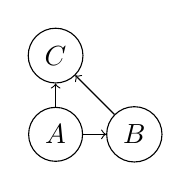
\begin{tikzpicture}[every node/.style={draw,circle}]
         \path (0,0) node (A) {$A$}
               (1,0) node (B) {$B$}
               (0,1) node (C) {$C$};
         \draw[->] (A) -- (B);
         \draw[->] (B) -- (C);
         \draw[->] (A) -- (C);
      \end{tikzpicture}
    \par
    \caption{Digraph for Question~\ref{ex:digraph}}
    \label{fig:digraph}
  \end{figure}
  \end{onlyproblem}
  \begin{onlysolution}
  $A$ is a souce and $C$ is a sink.
  \end{onlysolution}
\end{defproblem}
%    \end{macrocode}
%\fi
%\iffalse
%    \begin{macrocode}
%</prob-mixed.tex>
%    \end{macrocode}
%\fi
%\iffalse
%    \begin{macrocode}
%<*prob-newdata.tex>
%    \end{macrocode}
%\fi
%\iffalse
%    \begin{macrocode}
 % This file is public domain
\begin{defproblem}{sample}
\begin{onlyproblem}
Differentiate $y=\sin x$
\end{onlyproblem}
\begin{onlysolution}
$y'=\cos x$
\end{onlysolution}
\end{defproblem}

\begin{defproblem}[1]{sample2}
\begin{onlyproblem}
Differentiate $y = \sin(#1x)$
\end{onlyproblem}
\begin{onlysolution}
$y'=#1\cos #1x$
\end{onlysolution}
\end{defproblem}

\begin{defproblem}{sample3}
\begin{onlyproblem}
Differentiate $y = x^2$.
\end{onlyproblem}
\begin{onlysolution}
$y' = 2x$
\end{onlysolution}
\end{defproblem}
%    \end{macrocode}
%\fi
%\iffalse
%    \begin{macrocode}
%</prob-newdata.tex>
%    \end{macrocode}
%\fi
%\iffalse
%    \begin{macrocode}
%<*prob-nosoln.tex>
%    \end{macrocode}
%\fi
%\iffalse
%    \begin{macrocode}
 % This file is public domain
 %
 % these problems don't have solutions

\newproblem*{oop}{Describe what is meant by object-oriented
programming.}

\newproblem*{inheritance}{Describe what is meant by the term 
\emph{inheritance} in object-oriented programming. Use examples.}
%    \end{macrocode}
%\fi
%\iffalse
%    \begin{macrocode}
%</prob-nosoln.tex>
%    \end{macrocode}
%\fi
%\iffalse
%    \begin{macrocode}
%<*prob-probspaces.tex>
%    \end{macrocode}
%\fi
%\iffalse
%    \begin{macrocode}
 % This file is public domain
 %
 % Finite probability spaces
\newproblem{weightedcoin}{%
A coin is weighted so that heads is four times as likely
as tails. Find the probability that:
\begin{textenum}
\item tails appears,
\item heads appears
\end{textenum}}{%
Let $p=P(T)$, then $P(H)=4p$. We require $P(H)+P(T)=1$,
so $4p+p=1$, hence $p=\frac{1}{5}$. Therefore:
\begin{textenum}
\item $P(T)=\frac{1}{5}$,
\item $P(H)=\frac{4}{5}$
\end{textenum}}

\newproblem*{validprobspaces}{%
Under which of the following functions does 
$S=\{a_1,a_2\}$ become a probability space?
\par
\begin{textenum}
\begin{tabular}{ll}
\incorrectitem $P(a_1)=\frac{1}{3}$, $P(a_2)=\frac{1}{2}$
&
\correctitem $P(a_1)=\frac{3}{4}$, $P(a_2)=\frac{1}{4}$
\\
\correctitem $P(a_1)=1$, $P(a_2)=0$
&
\incorrectitem $P(a_1)=\frac{5}{4}$, $P(a_2)=-\frac{1}{4}$
\end{tabular}
\end{textenum}
}
%    \end{macrocode}
%\fi
%\iffalse
%    \begin{macrocode}
%</prob-probspaces.tex>
%    \end{macrocode}
%\fi
%\iffalse
%    \begin{macrocode}
%<*prob-probspaces2.tex>
%    \end{macrocode}
%\fi
%\iffalse
%    \begin{macrocode}
 % This file is public domain
 %
 % Finite probability spaces
\begin{defproblem}{weightedcoin}
\begin{onlyproblem}%
A coin is weighted so that heads is four times as likely
as tails. Find the probability that:
\begin{textenum}
\item tails appears,
\item heads appears
\end{textenum}
\end{onlyproblem}
\begin{onlysolution}%
Let $p=P(T)$, then $P(H)=4p$. We require $P(H)+P(T)=1$,
so $4p+p=1$, hence $p=\frac{1}{5}$. Therefore:
\begin{textenum}
\item $P(T)=\frac{1}{5}$,
\item $P(H)=\frac{4}{5}$
\end{textenum}
\end{onlysolution}
\end{defproblem}

\begin{defproblem}{validprobspaces}
\begin{onlyproblem}%
Under which of the following functions does 
$S=\{a_1,a_2\}$ become a probability space?
\par
\begin{textenum}
\begin{tabular}{ll}
\item $P(a_1)=\frac{1}{3}$, $P(a_2)=\frac{1}{2}$
&
\item\label{validprobspacescorrect1} $P(a_1)=\frac{3}{4}$, $P(a_2)=\frac{1}{4}$
\\
\item\label{validprobspacescorrect2} $P(a_1)=1$, $P(a_2)=0$
&
\item $P(a_1)=\frac{5}{4}$, $P(a_2)=-\frac{1}{4}$
\end{tabular}
\end{textenum}
\end{onlyproblem}%
\begin{onlysolution}%
\ref{validprobspacescorrect1} and \ref{validprobspacescorrect2}%
\end{onlysolution}
\end{defproblem}
%    \end{macrocode}
%\fi
%\iffalse
%    \begin{macrocode}
%</prob-probspaces2.tex>
%    \end{macrocode}
%\fi
%\iffalse
%    \begin{macrocode}
%<*prob-tabmchoice.tex>
%    \end{macrocode}
%\fi
%\iffalse
%    \begin{macrocode}
 % This file is public domain
 %
 % These problems are designed to be placed in a
 % tabular environment
 %
\newproblem{tab:1}{%
What is $(3+2)\times5$? &
25 \ifshowanswers\selected\else\notselected\fi &
13 \notselected &
10 \notselected &
}{Brackets come first}%

\newproblem{tab:2}{%
What is $-1+2\times3$? &
3 \notselected &
-7 \notselected &
5 \ifshowanswers\selected\else\notselected\fi &
}{Multiplication comes first}%
%    \end{macrocode}
%\fi
%\iffalse
%    \begin{macrocode}
%</prob-tabmchoice.tex>
%    \end{macrocode}
%\fi
%\iffalse
%    \begin{macrocode}
%<*prob-verb.tex>
%    \end{macrocode}
%\fi
%\iffalse
%    \begin{macrocode}
\begin{defproblem}{code-helloworld}
This problem has a code fragment.
\begin{onlyproblem}
\lstset{language=Java}
\begin{lstlisting}
public class HelloWorld
{
  public static void main(String[] args)
  {
     System.out.println("Hello World!");
  }
}
\end{lstlisting}
\end{onlyproblem}
\begin{onlysolution}
\lstset{language=Java}
\begin{lstlisting}
public class HelloWorld
{
  public static void main(String[] args)
  {
     System.out.println("Hello "
      + (args.length==0 ? "anon" : args[0])+"!");
  }
}
\end{lstlisting}
\end{onlysolution}
\end{defproblem}
%    \end{macrocode}
%\fi
%\iffalse
%    \begin{macrocode}
%</prob-verb.tex>
%    \end{macrocode}
%\fi
%\Finale
\endinput
